% =====================================================================
%  Chapter 15: Surfaces, Flux, Curl, and Divergence in Space
%  Sections 15.1 and 15.2
% =====================================================================

\chapter{Surfaces, Flux, Curl, and Divergence in Space}
\label{ch:15}

Chapter \ref{ch:14} ended with Green's theorem written in the compact form
\[
    \int_{\partial R}\omega=\int_R d\omega.
\]
There the region \(R\) was flat.  It lived in the \(xy\)-plane, and its boundary was a
closed curve.

But the formula itself did not look flat.  It spoke about a thing and its boundary.
That language wants to move into space.  A wire loop can bound a soap film.  A dome
has a rim.  A balloon has no rim, but it has an inside and an outside.  A river can flow
through a curved screen.

To carry Green's theorem into space, we first need to understand surfaces as objects
we can parametrize, measure, orient, and integrate over.

\section{Parametric surfaces and tangent planes}
\label{sec:15.1}

A curve needed one parameter:
\[
    \mathbf r(t).
\]
A surface needs two.  One parameter moves along one family of curves on the surface;
the other moves along a crossing family.  Together they form a coordinate grid on the
surface.

\subsection{Two parameters make a surface}

Think of a rectangular sheet of rubber.  Before it is bent, a point on the sheet can be
labeled by two numbers:
\[
    (u,v).
\]
After the sheet is bent into space, the point has three coordinates:
\[
    (x,y,z).
\]
So a bent sheet is naturally described by a function
\[
    \mathbf r(u,v)=(x(u,v),y(u,v),z(u,v)).
\]

The input \((u,v)\) lives in a flat parameter region.  The output \(\mathbf r(u,v)\)
lives in space.

For example, a cylinder of radius \(2\) can be described by
\[
    \mathbf r(\theta,z)=(2\cos\theta,\,2\sin\theta,\,z),
\]
where
\[
    0\le \theta\le 2\pi,
    \qquad
    0\le z\le 5.
\]
The parameter \(\theta\) moves around the cylinder.  The parameter \(z\) moves upward.

If \(\theta=\pi/3\) and \(z=4\), then
\[
    \mathbf r\left(\frac{\pi}{3},4\right)
    =
    \left(1,\sqrt3,4\right).
\]
So the flat rectangle
\[
    0\le \theta\le 2\pi,\qquad 0\le z\le5
\]
has been wrapped into the side of a cylinder.

\begin{figure}[h]
\centering
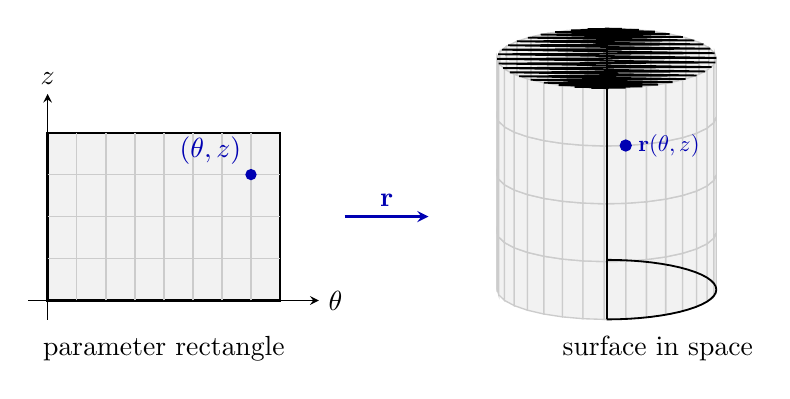
\begin{tikzpicture}[scale=0.82, >=stealth]
    % 1. Left side: Parameter Rectangle
    \begin{scope}
        \draw[->] (-0.3,0) -- (4.2,0) node[right] {\(\theta\)};
        \draw[->] (0,-0.3) -- (0,3.2) node[above] {\(z\)};
        \draw[fill=gray!10, thick] (0,0) rectangle (3.6,2.6);

        % Grid mathematically spaced to match the 3D geometry chunks
        \foreach \x in {0.45, 0.9, 1.35, 1.8, 2.25, 2.7, 3.15} {
            \draw[gray!40, semithick] (\x,0) -- (\x,2.6);
        }
        \foreach \y in {0.65,1.3,1.95} {
            \draw[gray!40, semithick] (0,\y) -- (3.6,\y);
        }

        % Picked a specific intersection (theta=315 degrees, z=1.95)
        \fill[blue!70!black] (3.15, 1.95) circle (2.5pt);
        \node[above left, blue!70!black] at (3.15, 1.95) {\((\theta,z)\)};

        \node at (1.8,-0.75) {parameter rectangle};
    \end{scope}

    % 2. Middle: Mapping Arrow
    \draw[->, thick, blue!70!black] (4.6,1.3) -- (5.9,1.3);
    \node[above, blue!70!black] at (5.25,1.3) {\(\mathbf r\)};

    % 3. Right side: Surface in Space (pgfplots)
    \begin{scope}[shift={(6.2,-0.5)}]
        \begin{axis}[
            width=6.5cm, height=6.5cm,
            view={35}{15},
            axis lines=none,
            z buffer=sort,
            clip=false,
            xmin=-1.3, xmax=1.3,
            ymin=-1.3, ymax=1.3,
            zmin=0, zmax=2.6
        ]
            % Main mathematical mesh surface
            \addplot3[
                surf,
                fill=gray!10,
                faceted color=gray!40,
                semithick,
                samples=33, samples y=5,
                domain=0:360, y domain=0:2.6
            ] ({1.25*cos(x)}, {1.25*sin(x)}, {y});

            % Crisp framing boundaries to give the shape defined edges
            % Top circle (fully visible)
            \addplot3[thick, draw=black, samples=41, domain=0:360] 
                ({1.25*cos(x)}, {1.25*sin(x)}, 2.6);
            % Bottom circle (only the visible front half from this view angle)
            \addplot3[thick, draw=black, samples=31, domain=-55:125] 
                ({1.25*cos(x)}, {1.25*sin(x)}, 0);
            % Left and right visual bounding lines
            \addplot3[thick, draw=black, samples=2] 
                coordinates {({1.25*cos(125)}, {1.25*sin(125)}, 0) ({1.25*cos(125)}, {1.25*sin(125)}, 2.6)};
            \addplot3[thick, draw=black, samples=2] 
                coordinates {({1.25*cos(305)}, {1.25*sin(305)}, 0) ({1.25*cos(305)}, {1.25*sin(305)}, 2.6)};

            % Highlighted mapped point in 3D
            \addplot3[only marks, mark=*, mark options={color=blue!70!black}, mark size=2.5pt] 
                coordinates {({1.25*cos(315)}, {1.25*sin(315)}, 1.95)};
            \node[right, xshift=2pt, blue!70!black] at (axis cs:{1.25*cos(315)}, {1.25*sin(315)}, 1.95) {\(\mathbf r(\theta,z)\)};

        \end{axis}
        \node at (3.25,-0.25) {surface in space};
    \end{scope}
\end{tikzpicture}
\caption{A parametrization turns a flat two-parameter region into a surface patch.}
\end{figure}

\begin{definition}[Parametric surface]
A \emph{parametric surface} in space is a function
\[
    \mathbf r:D\subseteq\mathbb R^2\to\mathbb R^3
\]
of the form
\[
    \mathbf r(u,v)=(x(u,v),y(u,v),z(u,v)).
\]
The set
\[
    \{\mathbf r(u,v):(u,v)\in D\}
\]
is the image of the parametrization.
\end{definition}

The parameters do not have to be called \(u\) and \(v\).  On a cylinder, it is more
natural to use \(\theta\) and \(z\).  On a sphere, it is more natural to use two angles.

\subsection{Coordinate curves on a surface}

A parametrized surface comes with two families of curves.

For the cylinder
\[
    \mathbf r(\theta,z)=(2\cos\theta,2\sin\theta,z),
\]
hold \(z\) fixed and let \(\theta\) vary.  We get a horizontal circle:
\[
    \theta\longmapsto (2\cos\theta,2\sin\theta,z_0).
\]
Hold \(\theta\) fixed and let \(z\) vary.  We get a vertical line:
\[
    z\longmapsto (2\cos\theta_0,2\sin\theta_0,z).
\]

These two curve families form the grid on the surface.

At a point, the derivatives of these coordinate curves give two tangent directions:
\[
    \mathbf r_\theta(\theta,z)=(-2\sin\theta,2\cos\theta,0),
\]
and
\[
    \mathbf r_z(\theta,z)=(0,0,1).
\]
At
\[
    \theta=\frac{\pi}{3},\qquad z=4,
\]
these become
\[
    \mathbf r_\theta\left(\frac{\pi}{3},4\right)=(-\sqrt3,1,0),
\]
and
\[
    \mathbf r_z\left(\frac{\pi}{3},4\right)=(0,0,1).
\]
One vector points around the cylinder.  The other points upward.

\begin{definition}[Tangent vectors from a parametrization]
Let
\[
    \mathbf r(u,v)=(x(u,v),y(u,v),z(u,v)).
\]
The two coordinate tangent vectors are
\[
\boxed{
    \mathbf r_u=(x_u,y_u,z_u),
    \qquad
    \mathbf r_v=(x_v,y_v,z_v).
}
\]
They are tangent to the coordinate curves obtained by holding one parameter fixed.
\end{definition}

A surface is locally two-dimensional when these two tangent directions are genuinely
different.  If one direction is a multiple of the other, the parameter grid has collapsed
at that point.

\subsection{Normal direction from the cross product}

Two nonparallel tangent vectors determine a plane.  A normal vector to that plane is
given by their cross product:
\[
    \mathbf r_u\times \mathbf r_v.
\]

For the cylinder,
\[
    \mathbf r_\theta=(-2\sin\theta,2\cos\theta,0),
    \qquad
    \mathbf r_z=(0,0,1).
\]
So
\[
\begin{aligned}
    \mathbf r_\theta\times \mathbf r_z
    &=
    (2\cos\theta,2\sin\theta,0).
\end{aligned}
\]
This vector points radially outward.  At \(\theta=\pi/3\),
\[
    \mathbf r_\theta\times \mathbf r_z=(1,\sqrt3,0).
\]
That is exactly the outward normal direction at the point
\[
    (1,\sqrt3,z).
\]

The order matters.  If we reverse the order,
\[
    \mathbf r_z\times \mathbf r_\theta
    =
    -(\mathbf r_\theta\times \mathbf r_z),
\]
so the normal points inward instead of outward.  This sign will become part of
orientation and flux later.

\begin{definition}[Smooth regular surface patch]
A parametrization
\[
    \mathbf r(u,v)
\]
is called \emph{smooth} if its first partial derivatives are continuous.

It is called \emph{regular} at \((u,v)\) if
\[
\boxed{
    \mathbf r_u(u,v)\times \mathbf r_v(u,v)\ne \mathbf 0.
}
\]
A smooth regular parametrization gives a smooth surface patch.
\end{definition}

The regularity condition says that the two parameter directions really make a little
surface patch, not just a curve or a point.

\subsection{Tangent planes to parametrized surfaces}

The tangent plane is the plane spanned by
\[
    \mathbf r_u(u_0,v_0)
    \qquad\text{and}\qquad
    \mathbf r_v(u_0,v_0).
\]
If
\[
    \mathbf p=\mathbf r(u_0,v_0),
\]
then a parametric equation for the tangent plane is
\[
\boxed{
    \mathbf X=\mathbf p+s\,\mathbf r_u(u_0,v_0)+t\,\mathbf r_v(u_0,v_0).
}
\]
A normal vector is
\[
    \mathbf n=\mathbf r_u(u_0,v_0)\times \mathbf r_v(u_0,v_0),
\]
so the same plane can be written as
\[
\boxed{
    \mathbf n\cdot(\mathbf X-\mathbf p)=0.
}
\]

\begin{theorem}[Tangent plane to a parametrized surface]
Let
\[
    \mathbf r:D\to\mathbb R^3
\]
be smooth and regular at \((u_0,v_0)\).  Set
\[
    \mathbf p=\mathbf r(u_0,v_0).
\]
Then the tangent plane to the surface at \(\mathbf p\) is
\[
\boxed{
    \mathbf X=\mathbf p+s\,\mathbf r_u(u_0,v_0)+t\,\mathbf r_v(u_0,v_0).
}
\]
Equivalently, if
\[
    \mathbf n=\mathbf r_u(u_0,v_0)\times \mathbf r_v(u_0,v_0),
\]
then
\[
\boxed{
    \mathbf n\cdot(\mathbf X-\mathbf p)=0.
}
\]
\end{theorem}

\begin{proof}
The curve
\[
    u\longmapsto \mathbf r(u,v_0)
\]
lies on the surface, and its velocity at \(u=u_0\) is
\[
    \mathbf r_u(u_0,v_0).
\]
So \(\mathbf r_u\) is tangent to the surface.

Similarly, the curve
\[
    v\longmapsto \mathbf r(u_0,v)
\]
lies on the surface, and its velocity at \(v=v_0\) is
\[
    \mathbf r_v(u_0,v_0).
\]
So \(\mathbf r_v\) is also tangent.

Regularity says these two directions are not parallel, so they span a plane.  Their
cross product is normal to that plane.
\end{proof}

\begin{example}[A tangent plane to a cylinder]
For the cylinder
\[
    \mathbf r(\theta,z)=(2\cos\theta,2\sin\theta,z),
\]
take
\[
    \theta=\frac{\pi}{3},
    \qquad
    z=4.
\]
Then
\[
    \mathbf p=(1,\sqrt3,4).
\]
The tangent vectors are
\[
    \mathbf r_\theta=(-\sqrt3,1,0),
    \qquad
    \mathbf r_z=(0,0,1).
\]
A normal vector is
\[
    \mathbf n=\mathbf r_\theta\times\mathbf r_z=(1,\sqrt3,0).
\]
Therefore the tangent plane is
\[
    (1,\sqrt3,0)\cdot\bigl((x,y,z)-(1,\sqrt3,4)\bigr)=0.
\]
That is
\[
    x-1+\sqrt3(y-\sqrt3)=0,
\]
or
\[
\boxed{
    x+\sqrt3\,y=4.
}
\]
The tangent plane is vertical, as it should be for the side of a cylinder.
\end{example}

\subsection{Graphs as parametrized surfaces}

A graph
\[
    z=g(x,y)
\]
is a surface.  It has the natural parametrization
\[
\boxed{
    \mathbf r(x,y)=(x,y,g(x,y)).
}
\]
The two tangent vectors are
\[
    \mathbf r_x=(1,0,g_x),
    \qquad
    \mathbf r_y=(0,1,g_y).
\]
Their cross product is
\[
\begin{aligned}
    \mathbf r_x\times \mathbf r_y
    &=
    (-g_x,-g_y,1).
\end{aligned}
\]
So a normal vector to the graph is
\[
\boxed{
    (-g_x,-g_y,1).
}
\]

This agrees with the tangent-plane formula from Chapter \ref{ch:9}.  If
\[
    \mathbf p=(a,b,g(a,b)),
\]
then
\[
    z-g(a,b)=g_x(a,b)(x-a)+g_y(a,b)(y-b).
\]

\begin{example}[A tangent plane to a curved shade cloth]
A shade cloth over a courtyard has height
\[
    g(x,y)=4+\frac{x}{3}-\frac{y}{4}-\frac{x^2}{12}.
\]
At the point
\[
    (x,y)=(1,2),
\]
the height is
\[
    g(1,2)
    =
    4+\frac13-\frac12-\frac1{12}
    =
    \frac{15}{4}.
\]
The partial derivatives are
\[
    g_x(x,y)=\frac13-\frac{x}{6},
    \qquad
    g_y(x,y)=-\frac14.
\]
At \((1,2)\),
\[
    g_x(1,2)=\frac16,
    \qquad
    g_y(1,2)=-\frac14.
\]
So the tangent plane is
\[
\boxed{
    z-\frac{15}{4}
    =
    \frac16(x-1)-\frac14(y-2).
}
\]
In parametric-surface language, this is the same plane spanned by
\[
    \mathbf r_x=\left(1,0,\frac16\right),
    \qquad
    \mathbf r_y=\left(0,1,-\frac14\right).
\]
\end{example}

\subsection{Why the hypotheses matter}

We asked for smoothness and regularity because tangent planes can fail in two different
ways.

First, a surface can have a crease.  Consider
\[
    z=|x|.
\]
A natural parametrization is
\[
    \mathbf r(x,y)=(x,y,|x|).
\]
Along the line \(x=0\), the surface folds like a roof ridge.  Approaching from \(x>0\),
the surface has slope \(+1\) in the \(x\)-direction.  Approaching from \(x<0\), it has
slope \(-1\).  There is no single tangent plane along the crease.

The partial derivative with respect to \(x\) does not exist there.  Smoothness was not
a decoration; it prevented a hidden fold.

Second, a parametrization can collapse.  A cone can be parametrized by
\[
    \mathbf r(u,\theta)=(u\cos\theta,u\sin\theta,u),
    \qquad
    u\ge0.
\]
The tangent vectors are
\[
    \mathbf r_u=(\cos\theta,\sin\theta,1),
\]
and
\[
    \mathbf r_\theta=(-u\sin\theta,u\cos\theta,0).
\]
Their cross product is
\[
    \mathbf r_u\times\mathbf r_\theta
    =
    (-u\cos\theta,-u\sin\theta,u).
\]
At the tip, where \(u=0\),
\[
    \mathbf r_u\times\mathbf r_\theta=\mathbf 0.
\]
The cone has no unique tangent plane at its tip.  Different straight lines on the cone
arrive at the tip with different tangent directions.  Regularity is the condition that
rules out this kind of collapse.

So a smooth regular patch is the surface version of a smooth curve with nonzero
velocity.  It has a well-defined tangent plane and a normal direction.

But a normal direction is not yet an area.  The vector
\[
    \mathbf r_u\times\mathbf r_v
\]
does two jobs at once: it points perpendicular to the surface, and its length measures
how much a tiny parameter rectangle has been stretched.  That length is the next
piece of the story.

\section{Surface area and scalar surface integrals}
\label{sec:15.2}

Section \ref{sec:15.1} gave us the two tangent vectors
\[
    \mathbf r_u,\qquad \mathbf r_v.
\]
Their cross product points normal to the surface.  Its length has another meaning:
it measures the area of the tiny parallelogram made by those two tangent vectors.

That is how surface area becomes a double integral.

\subsection{A small parameter rectangle becomes a small parallelogram}

Let
\[
    \mathbf r(u,v)
\]
be a smooth surface patch.  Take a tiny rectangle in the \((u,v)\)-plane with side
lengths
\[
    \Delta u,\qquad \Delta v.
\]
Near a point \((u_0,v_0)\), the two sides of its image are approximately
\[
    \mathbf r_u(u_0,v_0)\,\Delta u
\]
and
\[
    \mathbf r_v(u_0,v_0)\,\Delta v.
\]
So the tiny surface patch is approximately a parallelogram.

The area of a parallelogram spanned by vectors \(\mathbf a\) and \(\mathbf b\) is
\[
    \|\mathbf a\times\mathbf b\|.
\]
Therefore the tiny surface area is approximately
\[
\boxed{
    \Delta S
    \approx
    \|\mathbf r_u\times\mathbf r_v\|\,\Delta u\,\Delta v.
}
\]
In differential notation,
\[
\boxed{
    dS=\|\mathbf r_u\times\mathbf r_v\|\,du\,dv.
}
\]

\begin{figure}[h]
\centering
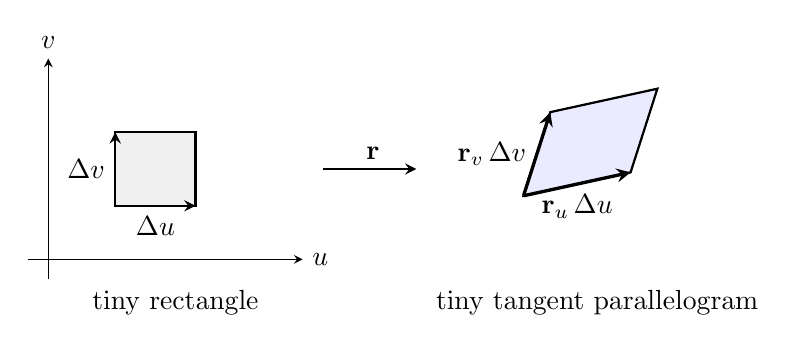
\begin{tikzpicture}[scale=0.85, >=stealth]
    \begin{scope}
        \draw[->] (-0.3,0) -- (3.8,0) node[right] {\(u\)};
        \draw[->] (0,-0.3) -- (0,3.0) node[above] {\(v\)};

        \draw[fill=gray!12, thick] (1,0.8) rectangle (2.2,1.9);
        \draw[->, thick] (1,0.8) -- (2.2,0.8) node[midway, below] {\(\Delta u\)};
        \draw[->, thick] (1,0.8) -- (1,1.9) node[midway, left] {\(\Delta v\)};

        \node at (1.9,-0.65) {tiny rectangle};
    \end{scope}

    \draw[->, thick] (4.1,1.35) -- (5.5,1.35);
    \node[above] at (4.85,1.35) {\(\mathbf r\)};

    \begin{scope}[shift={(6.3,0.15)}]
        \coordinate (P) at (0.8,0.8);
        \coordinate (A) at (2.4,1.15);
        \coordinate (B) at (1.2,2.05);
        \coordinate (C) at (2.8,2.4);

        \draw[fill=blue!8, thick] (P)--(A)--(C)--(B)--cycle;
        \draw[->, very thick] (P)--(A) node[midway, below] {\(\mathbf r_u\,\Delta u\)};
        \draw[->, very thick] (P)--(B) node[midway, left] {\(\mathbf r_v\,\Delta v\)};
        \draw[dashed] (A)--(C);
        \draw[dashed] (B)--(C);

        \node at (1.9,-0.8) {tiny tangent parallelogram};
    \end{scope}
\end{tikzpicture}
\caption{The area scale factor is \(\|\mathbf r_u\times\mathbf r_v\|\).}
\end{figure}

\subsection{Surface area from a parametrization}

If we add all the tiny surface pieces, we get surface area:
\[
    \sum \Delta S
    \approx
    \sum \|\mathbf r_u\times\mathbf r_v\|\,\Delta u\,\Delta v.
\]
Taking the limit gives the formula
\[
\boxed{
    \operatorname{Area}(S)
    =
    \iint_D \|\mathbf r_u\times\mathbf r_v\|\,du\,dv.
}
\]

\begin{example}[The side area of a cylinder]
The side of a cylinder of radius \(2\) and height \(5\) is parametrized by
\[
    \mathbf r(\theta,z)=(2\cos\theta,2\sin\theta,z),
\]
where
\[
    0\le\theta\le2\pi,
    \qquad
    0\le z\le5.
\]
We already computed
\[
    \mathbf r_\theta=(-2\sin\theta,2\cos\theta,0),
    \qquad
    \mathbf r_z=(0,0,1).
\]
Thus
\[
    \mathbf r_\theta\times\mathbf r_z
    =
    (2\cos\theta,2\sin\theta,0),
\]
and
\[
    \|\mathbf r_\theta\times\mathbf r_z\|=2.
\]
So
\[
\begin{aligned}
    \operatorname{Area}(S)
    &=
    \int_0^{2\pi}\int_0^5 2\,dz\,d\theta\\
    &=
    \int_0^{2\pi}10\,d\theta\\
    &=
    20\pi.
\end{aligned}
\]
This matches the familiar formula
\[
    \text{circumference}\times\text{height}
    =
    (4\pi)(5)=20\pi.
\]
\end{example}

The formula did not need us to remember the cylinder area formula.  It found the same
answer by measuring the stretching of the parameter rectangle.

\subsection{Scalar surface integrals}

Surface area adds
\[
    1\,dS
\]
over the surface.  If a quantity varies across the surface, we multiply by its value
before adding.

Suppose a thin shell has surface density
\[
    \sigma(x,y,z)
\]
in kilograms per square meter.  A small surface patch has mass approximately
\[
    \sigma(x,y,z)\,\Delta S.
\]
Adding gives
\[
    M=\iint_S \sigma\,dS.
\]

\begin{definition}[Scalar surface integral]
Let \(S\) be parametrized by a smooth regular map
\[
    \mathbf r:D\to\mathbb R^3
\]
that covers the surface once, except possibly along boundary curves.  For a scalar
function \(f\) on \(S\), the \emph{scalar surface integral} of \(f\) over \(S\) is
\[
\boxed{
    \iint_S f\,dS
    =
    \iint_D
    f(\mathbf r(u,v))\,
    \|\mathbf r_u(u,v)\times\mathbf r_v(u,v)\|\,
    du\,dv.
}
\]
When \(f=1\), this gives the surface area of \(S\).
\end{definition}

\begin{example}[Mass of a cylindrical shell]
A thin cylindrical shell has radius \(2\) and height \(5\).  Its density depends on height:
\[
    \sigma(x,y,z)=1+\frac{z}{10}
    \qquad \text{kg/m}^2.
\]
Using
\[
    \mathbf r(\theta,z)=(2\cos\theta,2\sin\theta,z),
\]
we have
\[
    dS=2\,d\theta\,dz.
\]
Therefore
\[
\begin{aligned}
M
&=
\int_0^{2\pi}\int_0^5
\left(1+\frac{z}{10}\right)2\,dz\,d\theta\\
&=
\int_0^{2\pi}
\left[
2z+\frac{z^2}{10}
\right]_0^5
\,d\theta\\
&=
\int_0^{2\pi}
\frac{25}{2}
\,d\theta\\
&=
25\pi.
\end{aligned}
\]
So the total mass is
\[
\boxed{
    M=25\pi\text{ kg}.
}
\]
\end{example}

A scalar surface integral does not care which side of the surface is chosen.  It uses
positive area.  That is why
\[
    \|\mathbf r_u\times\mathbf r_v\|
\]
appears, not the vector \(\mathbf r_u\times\mathbf r_v\) itself.

\subsection{Surface area of graphs}

For a graph
\[
    z=g(x,y),
\]
use the parametrization
\[
    \mathbf r(x,y)=(x,y,g(x,y)).
\]
Then
\[
    \mathbf r_x=(1,0,g_x),
    \qquad
    \mathbf r_y=(0,1,g_y).
\]
Their cross product is
\[
    \mathbf r_x\times \mathbf r_y=(-g_x,-g_y,1),
\]
so
\[
    \|\mathbf r_x\times \mathbf r_y\|
    =
    \sqrt{1+g_x^2+g_y^2}.
\]
Thus
\[
\boxed{
    dS=\sqrt{1+g_x^2+g_y^2}\,dx\,dy.
}
\]
For a graph over a region \(R\) in the \(xy\)-plane,
\[
\boxed{
    \operatorname{Area}(S)
    =
    \iint_R
    \sqrt{1+g_x^2+g_y^2}\,dA.
}
\]

\begin{example}[Area of a slanted roof]
A flat roof over the rectangle
\[
    0\le x\le6,
    \qquad
    0\le y\le4
\]
has height
\[
    z=2+\frac{x}{3}-\frac{y}{4}.
\]
Here
\[
    g_x=\frac13,
    \qquad
    g_y=-\frac14.
\]
So
\[
\sqrt{1+g_x^2+g_y^2}
=
\sqrt{1+\frac19+\frac1{16}}
=
\sqrt{\frac{169}{144}}
=
\frac{13}{12}.
\]
Therefore the roof area is
\[
\begin{aligned}
    \operatorname{Area}
    &=
    \int_0^6\int_0^4 \frac{13}{12}\,dy\,dx\\
    &=
    \frac{13}{12}\cdot24\\
    &=
    26.
\end{aligned}
\]
The flat floor area is \(24\).  The roof area is larger because the roof is tilted.
\end{example}

The formula
\[
    \sqrt{1+g_x^2+g_y^2}
\]
is the local stretching factor from the floor to the graph.  When the graph is nearly
flat, this factor is close to \(1\).  When the graph is steep, the surface uses more area
over the same floor region.

\subsection{Surface area in cylindrical and spherical coordinates}

Many surfaces are easiest to describe with cylindrical or spherical coordinates.

\subsubsection*{A horizontal disk}

A horizontal disk of radius \(a\) at height \(z=c\) can be parametrized by
\[
    \mathbf r(s,\theta)=(s\cos\theta,s\sin\theta,c),
\]
where
\[
    0\le s\le a,
    \qquad
    0\le\theta\le2\pi.
\]
Then
\[
    \mathbf r_s=(\cos\theta,\sin\theta,0),
\]
and
\[
    \mathbf r_\theta=(-s\sin\theta,s\cos\theta,0).
\]
So
\[
    \|\mathbf r_s\times\mathbf r_\theta\|=s.
\]
Thus
\[
\boxed{
    dS=s\,ds\,d\theta.
}
\]
This is the same area element used for polar coordinates in the plane.

\subsubsection*{The side of a cylinder}

A cylinder of radius \(a\) has parametrization
\[
    \mathbf r(\theta,z)=(a\cos\theta,a\sin\theta,z).
\]
Then
\[
    \|\mathbf r_\theta\times\mathbf r_z\|=a,
\]
so
\[
\boxed{
    dS=a\,d\theta\,dz.
}
\]

\subsubsection*{A sphere}

A sphere of radius \(a\) can be parametrized by
\[
    \mathbf r(\phi,\theta)
    =
    (a\sin\phi\cos\theta,\,
     a\sin\phi\sin\theta,\,
     a\cos\phi),
\]
where
\[
    0\le \phi\le\pi,
    \qquad
    0\le \theta\le2\pi.
\]
Here \(\phi\) is the angle down from the positive \(z\)-axis.

Compute:
\[
    \mathbf r_\phi
    =
    (a\cos\phi\cos\theta,\,
     a\cos\phi\sin\theta,\,
     -a\sin\phi),
\]
and
\[
    \mathbf r_\theta
    =
    (-a\sin\phi\sin\theta,\,
     a\sin\phi\cos\theta,\,
     0).
\]
A direct cross product gives
\[
    \|\mathbf r_\phi\times\mathbf r_\theta\|
    =
    a^2\sin\phi.
\]
Therefore
\[
\boxed{
    dS=a^2\sin\phi\,d\phi\,d\theta.
}
\]

The area of the sphere is then
\[
\begin{aligned}
    \operatorname{Area}
    &=
    \int_0^{2\pi}\int_0^\pi
    a^2\sin\phi\,d\phi\,d\theta\\
    &=
    \int_0^{2\pi}
    \left[-a^2\cos\phi\right]_0^\pi
    d\theta\\
    &=
    \int_0^{2\pi}2a^2\,d\theta\\
    &=
    4\pi a^2.
\end{aligned}
\]

At the poles, where \(\phi=0\) or \(\phi=\pi\), the factor
\[
    \sin\phi
\]
is \(0\).  The longitude lines all meet there, so the parametrization collapses in the
\(\theta\)-direction.  This is not a problem for the area integral because the collapse
happens only along the boundary of the parameter rectangle.  It would be a problem if
we tried to use one smooth regular patch containing the pole as an interior point.

\subsection{When parametrizations count too much}

The surface integral formula counts what the parametrization covers.

For the cylinder, if we used
\[
    0\le\theta\le4\pi
\]
instead of
\[
    0\le\theta\le2\pi,
\]
then the parametrization would wrap around the same cylinder twice.  The formula
would give
\[
    40\pi
\]
instead of
\[
    20\pi.
\]
The calculation is not broken.  It has computed the area with multiplicity.

This is why the definition said that the parametrization should cover the surface once,
except possibly along boundary curves.  When the same physical sheet is covered twice
by the parameter region, the integral counts it twice.

\subsection{Scalar area versus oriented area}

The scalar surface integral uses
\[
    dS=\|\mathbf r_u\times\mathbf r_v\|\,du\,dv.
\]
The norm removes the sign.  If we swap the order of the parameters, then
\[
    \mathbf r_v\times\mathbf r_u
    =
    -\mathbf r_u\times\mathbf r_v,
\]
but
\[
    \|\mathbf r_v\times\mathbf r_u\|
    =
    \|\mathbf r_u\times\mathbf r_v\|.
\]
So surface area and mass do not depend on which side of the surface we call positive.

That will change for flux.

If water flows through a net, it matters whether we count flow through the net upward
as positive or downward as positive.  The scalar area element \(dS\) cannot remember
that choice.  The full vector
\[
    \mathbf r_u\times\mathbf r_v
\]
can.

The same cross product that measured area has been quietly carrying orientation all
along.  Once we decide which side of a surface is positive, a surface integral can count
flow through the surface with a sign.  That signed quantity is called flux.
\section{Oriented surfaces and flux}
\label{sec:15.3}

Section \ref{sec:15.2} measured surface area with
\[
    dS=\|\mathbf r_u\times\mathbf r_v\|\,du\,dv.
\]
That formula deliberately forgot the sign of
\[
    \mathbf r_u\times\mathbf r_v.
\]
For mass and area, forgetting the sign was right.  But for flow through a surface, the
sign is the point.

A screen has two sides.  Water can pass through it one way or the other.  Air can move
from outside to inside or from inside to outside.  The same surface area is involved,
but the sign changes when we change which side we call positive.

\subsection{A surface has two normal directions}

Start with the simplest possible screen:
\[
    S=\{(x,y,1):0\le x\le2,\ 0\le y\le3\}.
\]
This is a horizontal rectangle at height \(z=1\).  Suppose air moves upward with
constant velocity
\[
    \mathbf F=(0,0,5).
\]
The surface has area
\[
    2\cdot3=6.
\]
If we choose the upward normal
\[
    \widehat{\mathbf n}=(0,0,1),
\]
then the air passes through the positive side of the screen at a rate
\[
    \mathbf F\cdot\widehat{\mathbf n}=5.
\]
So the total flow through the screen is
\[
    5\cdot6=30.
\]

If instead we choose the downward normal
\[
    \widehat{\mathbf n}=(0,0,-1),
\]
then
\[
    \mathbf F\cdot\widehat{\mathbf n}=-5,
\]
and the total flow is
\[
    -30.
\]

The physical motion did not change.  Only our choice of positive side changed.

\begin{figure}[h]
\centering
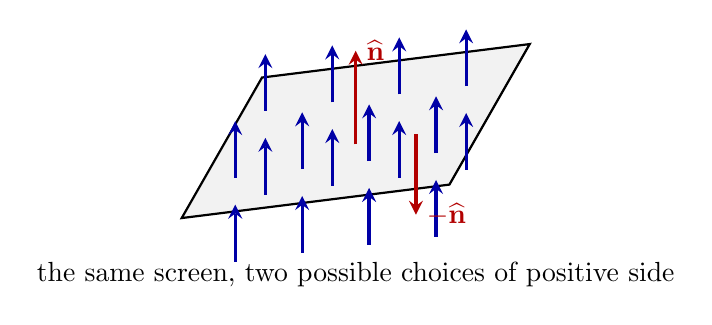
\begin{tikzpicture}[scale=0.85, >=stealth]
    \coordinate (A) at (0,0);
    \coordinate (B) at (4,0.5);
    \coordinate (C) at (5.2,2.6);
    \coordinate (D) at (1.2,2.1);

    \draw[fill=gray!10, thick] (A)--(B)--(C)--(D)--cycle;

    \foreach \x/\y in {0.8/0.35,1.8/0.48,2.8/0.60,3.8/0.72,1.25/1.35,2.25/1.48,3.25/1.60,4.25/1.72} {
        \draw[->, blue!65!black, very thick] (\x,\y-1.0) -- (\x,\y-0.15);
        \draw[->, blue!65!black, very thick] (\x,\y+0.25) -- (\x,\y+1.1);
    }

    \draw[->, red!70!black, very thick] (2.6,1.1) -- (2.6,2.5)
        node[right] {\(\widehat{\mathbf n}\)};
    \draw[->, red!70!black, very thick] (3.5,1.25) -- (3.5,0.05)
        node[right] {\(-\widehat{\mathbf n}\)};

    \node at (2.6,-0.85) {the same screen, two possible choices of positive side};
\end{tikzpicture}
\caption{Flux is signed.  Reversing the chosen normal reverses the sign.}
\end{figure}

\begin{definition}[Orientation of a surface]
An \emph{orientation} of a smooth surface is a continuous choice of unit normal vector
\[
    \widehat{\mathbf n}
\]
at each point of the surface.

A surface with such a continuous choice is called \emph{orientable}.
\end{definition}

For a parametrized surface
\[
    \mathbf r(u,v),
\]
the cross product
\[
    \mathbf r_u\times\mathbf r_v
\]
chooses a normal direction wherever it is nonzero.  The corresponding unit normal is
\[
\boxed{
    \widehat{\mathbf n}
    =
    \frac{\mathbf r_u\times\mathbf r_v}
    {\|\mathbf r_u\times\mathbf r_v\|}.
}
\]
If we swap the order of the parameters, the normal reverses:
\[
    \mathbf r_v\times\mathbf r_u
    =
    -\mathbf r_u\times\mathbf r_v.
\]

Not every surface can be oriented.  A M\"obius strip has only one side.  If you carry a
normal vector once around the strip, it comes back pointing the opposite way.  So there
is no continuous global choice of positive side.  We will return to this warning in
Section \ref{sec:15.8}.  For now, the surfaces we use will be orientable.

\subsection{Flux as signed flow through a surface}

Let
\[
    \mathbf F(x,y,z)
\]
be a vector field.  If \(\mathbf F\) is a fluid velocity field, then
\[
    \mathbf F\cdot\widehat{\mathbf n}
\]
measures the normal component of the velocity.

There are three possibilities:
\[
\begin{array}{c|c}
\mathbf F\cdot\widehat{\mathbf n}>0
&
\text{flow crosses in the positive normal direction}
\\[1mm]
\mathbf F\cdot\widehat{\mathbf n}<0
&
\text{flow crosses against the positive normal direction}
\\[1mm]
\mathbf F\cdot\widehat{\mathbf n}=0
&
\text{flow is tangent to the surface}
\end{array}
\]

A small surface patch has area approximately \(\Delta S\).  The amount of fluid crossing
it per unit time is approximately
\[
    \mathbf F\cdot\widehat{\mathbf n}\,\Delta S.
\]
Adding all patches gives the flux.

\begin{definition}[Flux integral]
Let \(S\) be an oriented smooth surface with chosen unit normal
\[
    \widehat{\mathbf n}.
\]
The \emph{flux} of a vector field \(\mathbf F\) through \(S\) is
\[
\boxed{
    \iint_S \mathbf F\cdot\widehat{\mathbf n}\,dS.
}
\]
\end{definition}

If \(\mathbf F\) is velocity measured in meters per second and \(dS\) is measured in
square meters, then flux has units
\[
    \frac{\text{m}}{\text{s}}\cdot \text{m}^2
    =
    \frac{\text{m}^3}{\text{s}}.
\]
So flux is volume per time.

\subsection{The vector area element}

The parametrization formula for flux comes from combining two things we already know:
\[
    dS=\|\mathbf r_u\times\mathbf r_v\|\,du\,dv
\]
and
\[
    \widehat{\mathbf n}
    =
    \frac{\mathbf r_u\times\mathbf r_v}
    {\|\mathbf r_u\times\mathbf r_v\|}.
\]
Multiplying them gives
\[
    \widehat{\mathbf n}\,dS
    =
    (\mathbf r_u\times\mathbf r_v)\,du\,dv.
\]
This vector
\[
    \widehat{\mathbf n}\,dS
\]
is called the \emph{oriented surface area element}.  It is area with a direction attached.

So, if the parametrization
\[
    \mathbf r(u,v)
\]
has the chosen orientation, then
\[
\boxed{
    \iint_S \mathbf F\cdot\widehat{\mathbf n}\,dS
    =
    \iint_D
    \mathbf F(\mathbf r(u,v))\cdot
    \bigl(\mathbf r_u\times\mathbf r_v\bigr)\,du\,dv.
}
\]
If \(\mathbf r_u\times\mathbf r_v\) points opposite to the chosen orientation, then the
right-hand side gives the negative of the desired flux.

\begin{theorem}[Flux through a parametrized surface]
Let
\[
    \mathbf r:D\to\mathbb R^3
\]
be a smooth regular parametrization that covers an oriented surface \(S\) once, except
possibly along boundary curves.  Suppose the chosen orientation is the one determined
by
\[
    \mathbf r_u\times\mathbf r_v.
\]
Then
\[
\boxed{
    \iint_S \mathbf F\cdot\widehat{\mathbf n}\,dS
    =
    \iint_D
    \mathbf F(\mathbf r(u,v))\cdot
    \bigl(\mathbf r_u\times\mathbf r_v\bigr)\,du\,dv.
}
\]
\end{theorem}

\begin{proof}
On a tiny parameter rectangle,
\[
    \Delta u\,\Delta v,
\]
the surface patch is approximately the parallelogram spanned by
\[
    \mathbf r_u\,\Delta u
    \qquad\text{and}\qquad
    \mathbf r_v\,\Delta v.
\]
Its oriented area vector is approximately
\[
    (\mathbf r_u\times\mathbf r_v)\,\Delta u\,\Delta v.
\]
The flux across that tiny patch is therefore approximately
\[
    \mathbf F(\mathbf r(u,v))\cdot
    (\mathbf r_u\times\mathbf r_v)\,\Delta u\,\Delta v.
\]
Adding these contributions and taking the limit gives the formula.
\end{proof}

The phrase ``covers once'' matters.  If a parametrization wraps around the same surface
twice, the flux integral counts the surface twice.  The calculation is not wrong; it is
computing flux with multiplicity.

\subsection{A slanted skylight in a steady wind}

A rectangular skylight lies in the plane
\[
    z=1+\frac{x}{2},
\]
above the rectangle
\[
    0\le x\le2,\qquad 0\le y\le3.
\]
Choose the upward orientation.  A steady wind is modeled by
\[
    \mathbf F=(2,1,5).
\]
Find the flux through the skylight.

Use the parametrization
\[
    \mathbf r(u,v)=\left(u,v,1+\frac u2\right),
    \qquad
    0\le u\le2,\quad 0\le v\le3.
\]
Then
\[
    \mathbf r_u=\left(1,0,\frac12\right),
    \qquad
    \mathbf r_v=(0,1,0).
\]
So
\[
\begin{aligned}
    \mathbf r_u\times\mathbf r_v
    &=
    \begin{vmatrix}
    \mathbf i&\mathbf j&\mathbf k\\
    1&0&1/2\\
    0&1&0
    \end{vmatrix}                                      \\[1mm]
    &=
    \left(-\frac12,0,1\right).
\end{aligned}
\]
This vector has positive \(z\)-component, so it gives the upward orientation.

The dot product is
\[
    \mathbf F\cdot(\mathbf r_u\times\mathbf r_v)
    =
    (2,1,5)\cdot\left(-\frac12,0,1\right)
    =
    -1+5
    =
    4.
\]
Therefore
\[
\begin{aligned}
    \iint_S \mathbf F\cdot\widehat{\mathbf n}\,dS
    &=
    \int_0^2\int_0^3 4\,dv\,du\\
    &=
    24.
\end{aligned}
\]
So the upward flux through the skylight is
\[
\boxed{
    24.
}
\]

The \(z\)-component of the wind contributes positively.  The \(x\)-component reduces
the flux because the upward normal leans slightly in the negative \(x\)-direction.

If we choose the downward orientation, the flux is
\[
    -24.
\]

\subsection{Flux through the side of a cylinder}

The side of a cylinder of radius \(a\) and height \(h\) is parametrized by
\[
    \mathbf r(\theta,z)=(a\cos\theta,a\sin\theta,z),
    \qquad
    0\le\theta\le2\pi,\quad 0\le z\le h.
\]
Then
\[
    \mathbf r_\theta=(-a\sin\theta,a\cos\theta,0),
    \qquad
    \mathbf r_z=(0,0,1).
\]
Their cross product is
\[
    \mathbf r_\theta\times\mathbf r_z
    =
    (a\cos\theta,a\sin\theta,0).
\]
This points outward.

Let
\[
    \mathbf F(x,y,z)=(x,y,0).
\]
On the cylinder,
\[
    \mathbf F(\mathbf r(\theta,z))=(a\cos\theta,a\sin\theta,0).
\]
Therefore
\[
\begin{aligned}
    \mathbf F(\mathbf r(\theta,z))\cdot
    (\mathbf r_\theta\times\mathbf r_z)
    &=
    (a\cos\theta,a\sin\theta,0)\cdot
    (a\cos\theta,a\sin\theta,0)\\
    &=
    a^2.
\end{aligned}
\]
So the outward flux through the side is
\[
\begin{aligned}
    \iint_S \mathbf F\cdot\widehat{\mathbf n}\,dS
    &=
    \int_0^{2\pi}\int_0^h a^2\,dz\,d\theta\\
    &=
    2\pi a^2h.
\end{aligned}
\]

For the cylinder of radius \(2\) and height \(5\),
\[
\boxed{
    \text{outward flux}=40\pi.
}
\]

Now compare this with the swirling field
\[
    \mathbf G(x,y,z)=(-y,x,0).
\]
On the cylinder,
\[
    \mathbf G(\mathbf r(\theta,z))=(-a\sin\theta,a\cos\theta,0).
\]
This is tangent to the cylinder.  Its dot product with the outward normal is
\[
    (-a\sin\theta,a\cos\theta,0)\cdot(a\cos\theta,a\sin\theta,0)=0.
\]
So
\[
\boxed{
    \iint_S \mathbf G\cdot\widehat{\mathbf n}\,dS=0.
}
\]
The field moves around the cylinder, not through it.

\subsection{Closed surfaces and outward orientation}

A surface with no boundary is called a \emph{closed surface}.  A sphere is closed.  The
boundary of a solid box is closed.  The side of a cylinder alone is not closed, because it
has two circular boundary curves.

For a closed surface, the standard orientation is the \emph{outward} orientation.

\begin{definition}[Outward orientation]
If \(S\) is the boundary of a solid region \(E\), the \emph{outward orientation} chooses
the normal direction that points away from the inside of \(E\).
\end{definition}

Flux through a closed surface measures net flow out of the region.  Flow leaving counts
positive.  Flow entering counts negative.

\begin{example}[A constant vertical field through a closed box]
Let \(B\) be a rectangular box, and let
\[
    \mathbf F=(0,0,5).
\]
The outward flux through the top face is positive.  The outward flux through the bottom
face is negative with the same magnitude.  The side faces have zero flux because the
field is tangent to them.

So the total outward flux is
\[
\boxed{
    0.
}
\]
The field passes through the box, but it does not create fluid inside the box.  Whatever
enters through the bottom leaves through the top.
\end{example}

\begin{example}[Outward flux through a sphere]
Let \(S\) be the sphere of radius \(a\) centered at the origin, with outward orientation.
Let
\[
    \mathbf F(x,y,z)=(x,y,z).
\]
At every point on the sphere,
\[
    \widehat{\mathbf n}=\frac{1}{a}(x,y,z).
\]
Thus
\[
    \mathbf F\cdot\widehat{\mathbf n}
    =
    (x,y,z)\cdot\frac{1}{a}(x,y,z)
    =
    \frac{x^2+y^2+z^2}{a}
    =
    a.
\]
Therefore
\[
\begin{aligned}
    \iint_S \mathbf F\cdot\widehat{\mathbf n}\,dS
    &=
    \iint_S a\,dS\\
    &=
    a\cdot 4\pi a^2\\
    &=
    4\pi a^3.
\end{aligned}
\]
So
\[
\boxed{
    \iint_S (x,y,z)\cdot\widehat{\mathbf n}\,dS=4\pi a^3.
}
\]
The field points outward everywhere, and its strength grows with radius.
\end{example}

Flux is now a surface integral with a sign.  But the formula
\[
    \mathbf F\cdot(\mathbf r_u\times\mathbf r_v)
\]
still hides something.  The cross product has three components:
\[
    y_u z_v-y_v z_u,
    \qquad
    z_u x_v-z_v x_u,
    \qquad
    x_u y_v-x_v y_u.
\]
Each one is a signed area of a shadow on a coordinate plane.  That is exactly the kind
of measurement that wedge products were built to remember.  The next step is to write
flux without hiding those signed areas inside a cross product.

\section{Flux \texorpdfstring{\(2\)}{2}-forms}
\label{sec:15.4}

The flux formula from Section \ref{sec:15.3} is
\[
    \iint_S \mathbf F\cdot\widehat{\mathbf n}\,dS
    =
    \iint_D
    \mathbf F(\mathbf r(u,v))\cdot
    \bigl(\mathbf r_u\times\mathbf r_v\bigr)\,du\,dv.
\]
This is efficient, but it hides the signed-area pieces.  In Chapter \ref{ch:14}, the form
\[
    dx\wedge dy
\]
measured oriented area in the \(xy\)-plane.  A surface in space has three coordinate
shadows, so flux needs three oriented area forms:
\[
    dy\wedge dz,\qquad dz\wedge dx,\qquad dx\wedge dy.
\]

\subsection{A wall perpendicular to the \(x\)-axis}

Take a flat wall
\[
    x=2,\qquad 0\le y\le3,\qquad 0\le z\le4.
\]
Orient it in the positive \(x\)-direction.  A natural parametrization is
\[
    \mathbf r(y,z)=(2,y,z).
\]
Then
\[
    \mathbf r_y=(0,1,0),
    \qquad
    \mathbf r_z=(0,0,1),
\]
so
\[
    \mathbf r_y\times\mathbf r_z=(1,0,0).
\]
For a vector field
\[
    \mathbf F=(P,Q,R),
\]
the flux through this wall is
\[
\begin{aligned}
    \iint_S \mathbf F\cdot\widehat{\mathbf n}\,dS
    &=
    \int_0^3\int_0^4
    \mathbf F(2,y,z)\cdot(1,0,0)\,dz\,dy\\
    &=
    \int_0^3\int_0^4 P(2,y,z)\,dz\,dy.
\end{aligned}
\]
Only the \(x\)-component of the field crosses a wall whose positive normal points in
the \(x\)-direction.

The area element on this wall is
\[
    dy\wedge dz.
\]
So the flux integrand is
\[
    P\,dy\wedge dz.
\]

The other coordinate walls follow the same pattern.

\[
\begin{array}{c|c|c}
\text{positive normal direction} & \text{ordered tangent directions} & \text{oriented area form}\\ \hline
\mathbf i & \mathbf j,\mathbf k & dy\wedge dz\\[1mm]
\mathbf j & \mathbf k,\mathbf i & dz\wedge dx\\[1mm]
\mathbf k & \mathbf i,\mathbf j & dx\wedge dy
\end{array}
\]

The middle entry
\[
    dz\wedge dx
\]
is not a typo.  The ordered directions
\[
    \mathbf k,\mathbf i
\]
have cross product
\[
    \mathbf k\times\mathbf i=\mathbf j.
\]
That is the positive \(y\)-normal.

\subsection{The flux form of a vector field}

The coordinate-wall computation suggests the right \(2\)-form.

\begin{definition}[Flux \(2\)-form]
Let
\[
    \mathbf F=(P,Q,R)
\]
be a vector field in space.  The \emph{flux \(2\)-form} associated to \(\mathbf F\) is
\[
\boxed{
    \Phi_{\mathbf F}
    =
    P\,dy\wedge dz
    +
    Q\,dz\wedge dx
    +
    R\,dx\wedge dy.
}
\]
\end{definition}

This form packages the three possible coordinate fluxes:
\[
\begin{array}{c|c}
\text{field component} & \text{oriented coordinate area it crosses} \\ \hline
P & dy\wedge dz\\[1mm]
Q & dz\wedge dx\\[1mm]
R & dx\wedge dy
\end{array}
\]

So the vector field
\[
    \mathbf F=(P,Q,R)
\]
and the \(2\)-form
\[
    \Phi_{\mathbf F}
\]
carry the same flux information.

\subsection{The shadows of a surface patch}

The formula
\[
    P\,dy\wedge dz
    +
    Q\,dz\wedge dx
    +
    R\,dx\wedge dy
\]
is easier to trust after seeing what it does to one tiny surface patch.

Let
\[
    \mathbf a=(a_1,a_2,a_3),
    \qquad
    \mathbf b=(b_1,b_2,b_3)
\]
be two tangent vectors spanning a tiny oriented parallelogram.  The form
\[
    dy\wedge dz
\]
measures the signed area of the shadow of this parallelogram on the \(yz\)-plane:
\[
    (dy\wedge dz)(\mathbf a,\mathbf b)
    =
    \begin{vmatrix}
    a_2&b_2\\
    a_3&b_3
    \end{vmatrix}
    =
    a_2b_3-a_3b_2.
\]
Similarly,
\[
    (dz\wedge dx)(\mathbf a,\mathbf b)
    =
    a_3b_1-a_1b_3,
\]
and
\[
    (dx\wedge dy)(\mathbf a,\mathbf b)
    =
    a_1b_2-a_2b_1.
\]
But these three numbers are exactly the components of the cross product:
\[
\boxed{
    \mathbf a\times\mathbf b
    =
    \bigl(
    (dy\wedge dz)(\mathbf a,\mathbf b),\,
    (dz\wedge dx)(\mathbf a,\mathbf b),\,
    (dx\wedge dy)(\mathbf a,\mathbf b)
    \bigr).
}
\]
Therefore
\[
\begin{aligned}
    \Phi_{\mathbf F}(\mathbf a,\mathbf b)
    &=
    P(dy\wedge dz)(\mathbf a,\mathbf b)
    +
    Q(dz\wedge dx)(\mathbf a,\mathbf b)\\
    &\qquad
    +
    R(dx\wedge dy)(\mathbf a,\mathbf b)\\
    &=
    (P,Q,R)\cdot(\mathbf a\times\mathbf b)\\
    &=
    \mathbf F\cdot(\mathbf a\times\mathbf b).
\end{aligned}
\]
So the flux \(2\)-form is not a new kind of flux.  It is the same flux, written as a
signed-area measurement.

\subsection{Pulling a \(2\)-form back to a parameter domain}

Let
\[
    \mathbf r(u,v)=(x(u,v),y(u,v),z(u,v))
\]
parametrize an oriented surface.  To integrate a \(2\)-form over this surface, we rewrite
the form in terms of \(du\) and \(dv\).  This substitution is called a \emph{pullback}.

The coordinate differentials become
\[
    dx=x_u\,du+x_v\,dv,
\]
\[
    dy=y_u\,du+y_v\,dv,
\]
and
\[
    dz=z_u\,du+z_v\,dv.
\]
Now compute:
\[
\begin{aligned}
    dy\wedge dz
    &=
    (y_u\,du+y_v\,dv)\wedge(z_u\,du+z_v\,dv)\\
    &=
    (y_u z_v-y_v z_u)\,du\wedge dv.
\end{aligned}
\]
Similarly,
\[
    dz\wedge dx
    =
    (z_u x_v-z_v x_u)\,du\wedge dv,
\]
and
\[
    dx\wedge dy
    =
    (x_u y_v-x_v y_u)\,du\wedge dv.
\]

Thus the flux form pulls back to
\[
\boxed{
\begin{aligned}
    \mathbf r^*\Phi_{\mathbf F}
    &=
    \Bigl[
    P(\mathbf r)(y_u z_v-y_v z_u)
    +
    Q(\mathbf r)(z_u x_v-z_v x_u)\\
    &\qquad
    +
    R(\mathbf r)(x_u y_v-x_v y_u)
    \Bigr]\,du\wedge dv.
\end{aligned}
}
\]
The coefficient in brackets is exactly
\[
    \mathbf F(\mathbf r(u,v))\cdot
    \bigl(\mathbf r_u\times\mathbf r_v\bigr).
\]

\begin{definition}[Surface integral of a \(2\)-form]
Let \(S\) be an oriented surface parametrized by
\[
    \mathbf r:D\to\mathbb R^3
\]
with the orientation determined by \(\mathbf r_u\times\mathbf r_v\).  If
\[
    \mathbf r^*\Phi=A(u,v)\,du\wedge dv,
\]
then
\[
\boxed{
    \iint_S \Phi
    =
    \iint_D A(u,v)\,du\,dv.
}
\]
\end{definition}

For a flux form,
\[
\boxed{
    \iint_S \Phi_{\mathbf F}
    =
    \iint_S \mathbf F\cdot\widehat{\mathbf n}\,dS.
}
\]
The two notations describe the same signed surface integral.

Reversing the orientation reverses the sign.  Covering the same surface twice doubles
the integral.  These are not defects of the formula; they are reminders that \(2\)-form
integrals are integrals over oriented surfaces.

\subsection{The slanted skylight again}

Return to the skylight
\[
    z=1+\frac{x}{2},
    \qquad
    0\le x\le2,\quad 0\le y\le3,
\]
with upward orientation, and the vector field
\[
    \mathbf F=(2,1,5).
\]
The flux form is
\[
    \Phi_{\mathbf F}
    =
    2\,dy\wedge dz
    +
    dz\wedge dx
    +
    5\,dx\wedge dy.
\]

Use the parametrization
\[
    \mathbf r(u,v)=\left(u,v,1+\frac u2\right).
\]
Then
\[
    dx=du,\qquad dy=dv,\qquad dz=\frac12\,du.
\]
Pull back each term:
\[
    dy\wedge dz
    =
    dv\wedge\frac12du
    =
    -\frac12\,du\wedge dv,
\]
\[
    dz\wedge dx
    =
    \frac12du\wedge du
    =
    0,
\]
and
\[
    dx\wedge dy
    =
    du\wedge dv.
\]
Therefore
\[
\begin{aligned}
    \mathbf r^*\Phi_{\mathbf F}
    &=
    2\left(-\frac12\,du\wedge dv\right)
    +
    0
    +
    5\,du\wedge dv\\
    &=
    4\,du\wedge dv.
\end{aligned}
\]
So
\[
\begin{aligned}
    \iint_S \Phi_{\mathbf F}
    &=
    \int_0^2\int_0^3 4\,dv\,du\\
    &=
    24.
\end{aligned}
\]
This matches the cross-product computation from Section \ref{sec:15.3}.

The form calculation shows where the number \(4\) came from:
\[
    5\,dx\wedge dy
\]
gave the upward contribution, while
\[
    2\,dy\wedge dz
\]
subtracted \(1\) because the skylight has a \(yz\)-shadow with the opposite sign.

\subsection{Graphs and a useful flux formula}

For a graph
\[
    z=g(x,y),
\]
use the upward orientation and the parametrization
\[
    \mathbf r(x,y)=(x,y,g(x,y)).
\]
Then
\[
    dz=g_x\,dx+g_y\,dy.
\]
Pull back the flux form
\[
    \Phi_{\mathbf F}
    =
    P\,dy\wedge dz
    +
    Q\,dz\wedge dx
    +
    R\,dx\wedge dy.
\]
We get
\[
    dy\wedge dz
    =
    dy\wedge(g_x\,dx+g_y\,dy)
    =
    -g_x\,dx\wedge dy,
\]
and
\[
    dz\wedge dx
    =
    (g_x\,dx+g_y\,dy)\wedge dx
    =
    -g_y\,dx\wedge dy.
\]
Therefore
\[
\boxed{
    \mathbf r^*\Phi_{\mathbf F}
    =
    \bigl(-P g_x-Q g_y+R\bigr)\,dx\wedge dy,
}
\]
where \(P,Q,R\) are evaluated at
\[
    (x,y,g(x,y)).
\]
So the upward flux through a graph is
\[
\boxed{
    \iint_S \mathbf F\cdot\widehat{\mathbf n}\,dS
    =
    \iint_R
    \bigl(-P(x,y,g)g_x-Q(x,y,g)g_y+R(x,y,g)\bigr)\,dx\,dy.
}
\]

This is the same as the cross-product formula, because
\[
    \mathbf r_x\times\mathbf r_y=(-g_x,-g_y,1).
\]

\subsection{A cylinder in flux-form language}

Let
\[
    \mathbf F(x,y,z)=(x,y,0).
\]
Then
\[
    \Phi_{\mathbf F}
    =
    x\,dy\wedge dz
    +
    y\,dz\wedge dx.
\]
Parametrize the outward-oriented side of the cylinder of radius \(a\) and height \(h\) by
\[
    \mathbf r(\theta,z)=(a\cos\theta,a\sin\theta,z),
    \qquad
    0\le\theta\le2\pi,\quad 0\le z\le h.
\]
Then
\[
    x=a\cos\theta,
    \qquad
    y=a\sin\theta,
\]
and
\[
    dx=-a\sin\theta\,d\theta,
    \qquad
    dy=a\cos\theta\,d\theta.
\]
So
\[
    dy\wedge dz
    =
    a\cos\theta\,d\theta\wedge dz,
\]
and
\[
\begin{aligned}
    dz\wedge dx
    &=
    dz\wedge(-a\sin\theta\,d\theta)\\
    &=
    a\sin\theta\,d\theta\wedge dz.
\end{aligned}
\]
Pull back the flux form:
\[
\begin{aligned}
    \mathbf r^*\Phi_{\mathbf F}
    &=
    a\cos\theta
    \bigl(a\cos\theta\,d\theta\wedge dz\bigr)
    +
    a\sin\theta
    \bigl(a\sin\theta\,d\theta\wedge dz\bigr)\\
    &=
    a^2(\cos^2\theta+\sin^2\theta)\,d\theta\wedge dz\\
    &=
    a^2\,d\theta\wedge dz.
\end{aligned}
\]
Thus
\[
\begin{aligned}
    \iint_S \Phi_{\mathbf F}
    &=
    \int_0^{2\pi}\int_0^h a^2\,dz\,d\theta\\
    &=
    2\pi a^2h.
\end{aligned}
\]
Again, this matches the classical flux calculation.

\subsection{Why the \(2\)-form notation matters}

The cross product is fast in \(\mathbb R^3\).  The flux \(2\)-form is more revealing.

It says that flux is built from three signed shadows:
\[
\boxed{
    \Phi_{\mathbf F}
    =
    P\,dy\wedge dz
    +
    Q\,dz\wedge dx
    +
    R\,dx\wedge dy.
}
\]
The \(P\)-component crosses \(yz\)-area, the \(Q\)-component crosses \(zx\)-area, and
the \(R\)-component crosses \(xy\)-area.

This form notation also prepares the next theorem.  In the plane, Green's theorem said
\[
    \int_{\partial R}\omega=\int_R d\omega.
\]
The derivative of a plane \(1\)-form became a \(2\)-form:
\[
    d(P\,dx+Q\,dy)=(Q_x-P_y)\,dx\wedge dy.
\]
In space, the derivative of a \(1\)-form also becomes a \(2\)-form, but now it has three
pieces:
\[
\begin{aligned}
d(P\,dx+Q\,dy+R\,dz)
&=
(R_y-Q_z)\,dy\wedge dz\\
&\quad+
(P_z-R_x)\,dz\wedge dx\\
&\quad+
(Q_x-P_y)\,dx\wedge dy.
\end{aligned}
\]
Those three coefficients form a vector.  That vector is called the curl.

So the next surface integral will look like flux, but it will come from circulation around
a boundary curve.  A wire loop can bound many different surfaces, and the same
boundary integral will know how much curl passes through any one of them.
\section{Curl and Stokes' theorem}
\label{sec:15.5}

Section \ref{sec:15.4} turned flux into a \(2\)-form:
\[
    \Phi_{\mathbf F}
    =
    P\,dy\wedge dz
    +
    Q\,dz\wedge dx
    +
    R\,dx\wedge dy.
\]
At the end, a different kind of \(2\)-form appeared.  If
\[
    \omega=P\,dx+Q\,dy+R\,dz
\]
is a work \(1\)-form, then \(d\omega\) is also a \(2\)-form.  Its three coefficients form
a vector.  That vector is called the \emph{curl}.

The meaning is simple but deep: curl measures local circulation per unit area.

\subsection{A small paddle wheel in space}

Picture a tiny paddle wheel floating in a moving fluid.  If the fluid pushes harder on
one side than the other, the wheel spins.  In the plane, Chapter \ref{ch:14} measured
this tendency with the scalar curl
\[
    Q_x-P_y.
\]
In space, the paddle wheel can face many directions.  A wheel lying flat in the
\(xy\)-plane detects spinning around the \(z\)-axis.  A wheel in the \(yz\)-plane detects
spinning around the \(x\)-axis.  A wheel in the \(zx\)-plane detects spinning around
the \(y\)-axis.

So curl in space needs three components.

Start with a vector field
\[
    \mathbf F=(P,Q,R)
\]
and its work form
\[
    \omega=P\,dx+Q\,dy+R\,dz.
\]

On a tiny rectangle in the \(xy\)-plane, the circulation density is
\[
    Q_x-P_y.
\]
That is the \(z\)-component of curl.

On a tiny rectangle in the \(yz\)-plane, the positive normal direction is the
\(x\)-direction.  The relevant work form is
\[
    Q\,dy+R\,dz.
\]
By the same rectangle argument as in Chapter \ref{ch:14}, the circulation density is
\[
    R_y-Q_z.
\]
That is the \(x\)-component of curl.

On a tiny rectangle whose ordered area form is
\[
    dz\wedge dx,
\]
the positive normal direction is the \(y\)-direction, because
\[
    \mathbf k\times \mathbf i=\mathbf j.
\]
The relevant circulation density is
\[
    P_z-R_x.
\]
That is the \(y\)-component of curl.

\[
\begin{array}{c|c|c}
\text{oriented coordinate area} & \text{positive normal} & \text{circulation density}\\ \hline
dy\wedge dz & \mathbf i & R_y-Q_z\\[1mm]
dz\wedge dx & \mathbf j & P_z-R_x\\[1mm]
dx\wedge dy & \mathbf k & Q_x-P_y
\end{array}
\]

These three numbers form one vector.

\begin{definition}[Curl]
Let
\[
    \mathbf F=(P,Q,R)
\]
be a vector field in space.  The \emph{curl} of \(\mathbf F\) is
\[
\boxed{
    \nabla\times \mathbf F
    =
    (R_y-Q_z,\;P_z-R_x,\;Q_x-P_y).
}
\]
\end{definition}

The notation
\[
    \nabla\times\mathbf F
\]
is classical vector notation.  It is useful, but it hides the form story.  The form story
says that curl is the vector field whose flux \(2\)-form is \(d\omega\).

Indeed, compute:
\[
\begin{aligned}
d(P\,dx+Q\,dy+R\,dz)
&=
dP\wedge dx+dQ\wedge dy+dR\wedge dz\\
&=
(R_y-Q_z)\,dy\wedge dz\\
&\quad+
(P_z-R_x)\,dz\wedge dx\\
&\quad+
(Q_x-P_y)\,dx\wedge dy.
\end{aligned}
\]
So
\[
\boxed{
    d\omega
    =
    \Phi_{\nabla\times\mathbf F}.
}
\]
In words:

\[
\boxed{
    \text{the exterior derivative of the work form is the flux form of the curl.}
}
\]

This is the bridge between circulation and flux.

\subsection{A first Stokes calculation: a circular wire}

Let
\[
    \mathbf F(x,y,z)=\left(-\frac y2,\frac x2,0\right),
\]
so
\[
    \omega=-\frac y2\,dx+\frac x2\,dy.
\]
The curl is
\[
\begin{aligned}
\nabla\times\mathbf F
&=
(0-0,\;0-0,\;\frac12-(-\frac12))\\
&=
(0,0,1).
\end{aligned}
\]
Equivalently,
\[
    d\omega=dx\wedge dy.
\]

Let \(C\) be the circle of radius \(a\) in the plane \(z=0\), oriented counterclockwise
as seen from above:
\[
    \mathbf r(t)=(a\cos t,a\sin t,0),
    \qquad 0\le t\le 2\pi.
\]
Then
\[
    dx=-a\sin t\,dt,
    \qquad
    dy=a\cos t\,dt.
\]
Pull back \(\omega\):
\[
\begin{aligned}
\omega
&=
-\frac{a\sin t}{2}(-a\sin t\,dt)
+
\frac{a\cos t}{2}(a\cos t\,dt)\\
&=
\frac{a^2}{2}(\sin^2t+\cos^2t)\,dt\\
&=
\frac{a^2}{2}\,dt.
\end{aligned}
\]
Therefore
\[
\begin{aligned}
\oint_C \omega
&=
\int_0^{2\pi}\frac{a^2}{2}\,dt\\
&=
\pi a^2.
\end{aligned}
\]

Now let \(D\) be the flat disk bounded by \(C\), with upward orientation.  Since
\[
    d\omega=dx\wedge dy,
\]
we get
\[
\begin{aligned}
\iint_D d\omega
&=
\iint_D dx\wedge dy\\
&=
\operatorname{Area}(D)\\
&=
\pi a^2.
\end{aligned}
\]
So
\[
\boxed{
    \oint_C \omega=\iint_D d\omega.
}
\]

In classical vector notation, the same statement is
\[
\boxed{
    \oint_C \mathbf F\cdot d\mathbf r
    =
    \iint_D (\nabla\times\mathbf F)\cdot\widehat{\mathbf n}\,dS.
}
\]

The left side walks around the wire.  The right side measures how much curl passes
through a surface spanning the wire.

\subsection{Surface orientation and boundary orientation}

A surface orientation chooses a normal direction.  Once that normal is chosen, the
positive direction around the boundary is forced.

For a parametrized surface
\[
    \mathbf r(u,v)
\]
whose orientation is given by
\[
    \mathbf r_u\times\mathbf r_v,
\]
the boundary orientation is the image of the positive boundary orientation of the
parameter region.  This is the most reliable rule.

There is also a hand rule.  Point the thumb of your right hand in the chosen normal
direction.  Your curled fingers show the positive boundary direction.

For a flat disk with upward normal, the boundary is counterclockwise as seen from
above.  If the same disk is oriented downward, the positive boundary direction is
clockwise.

\begin{figure}[h]
\centering
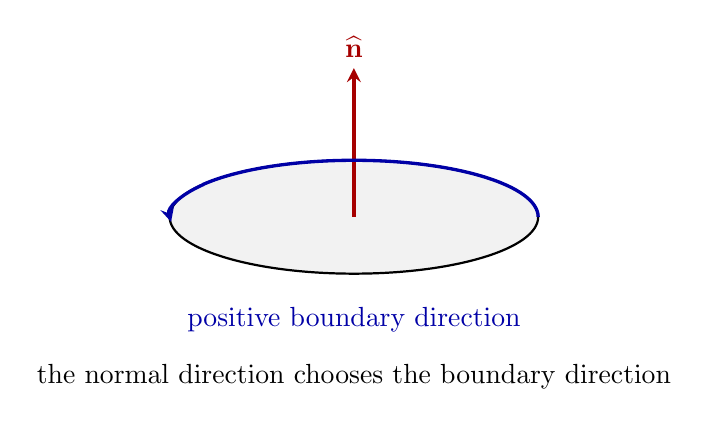
\begin{tikzpicture}[scale=0.9, >=stealth]
    \draw[fill=gray!10, thick] (0,0) ellipse (2.6 and 0.8);

    \draw[->, very thick, red!65!black] (0,0) -- (0,2.1)
        node[above] {\(\widehat{\mathbf n}\)};

    \draw[very thick, blue!65!black] (2.6,0) arc[start angle=0,end angle=145,x radius=2.6,y radius=0.8];
    \draw[->, very thick, blue!65!black] (-2.12,0.46) arc[start angle=145,end angle=185,x radius=2.6,y radius=0.8];

    \node[blue!65!black] at (0,-1.45) {positive boundary direction};

    \node at (0,-2.25) {the normal direction chooses the boundary direction};
\end{tikzpicture}
\caption{For Stokes' theorem, the surface orientation and boundary orientation must
match.}
\end{figure}

\begin{definition}[Compatible boundary orientation]
Let \(S\) be an oriented surface with boundary \(\partial S\).  The boundary is given
the \emph{compatible orientation} if, near each boundary point, the surface lies on the
left as seen from the chosen positive side of the surface.

Equivalently, for a parametrized oriented surface, \(\partial S\) receives the orientation
induced from the positively oriented boundary of the parameter domain.
\end{definition}

This compatibility is not bookkeeping.  It controls the sign of the theorem.

\subsection{Stokes' theorem}

The circle computation was not a coincidence.  It is the space version of Green's
theorem.

\begin{theorem}[Stokes' theorem]
Let \(S\) be an oriented piecewise smooth surface with piecewise smooth boundary
\[
    \partial S.
\]
Let
\[
    \mathbf F=(P,Q,R)
\]
have continuous first partial derivatives on an open region containing \(S\).  Give
\(\partial S\) the orientation compatible with the chosen orientation of \(S\).  Then
\[
\boxed{
    \oint_{\partial S}\mathbf F\cdot d\mathbf r
    =
    \iint_S(\nabla\times\mathbf F)\cdot\widehat{\mathbf n}\,dS.
}
\]
In differential-form notation, if
\[
    \omega=P\,dx+Q\,dy+R\,dz,
\]
then
\[
\boxed{
    \int_{\partial S}\omega
    =
    \int_S d\omega.
}
\]
\end{theorem}

\begin{proof}[Proof idea]
Parametrize the surface by
\[
    \mathbf r:D\to S,
\]
with orientation given by
\[
    \mathbf r_u\times\mathbf r_v.
\]
The boundary of \(S\) is the image of the boundary of \(D\), with the induced
orientation.

Pull the \(1\)-form \(\omega\) back to the parameter domain:
\[
    \mathbf r^*\omega.
\]
This is now a \(1\)-form on a region in the \(uv\)-plane.  By Green's theorem,
\[
    \int_{\partial D}\mathbf r^*\omega
    =
    \int_D d(\mathbf r^*\omega).
\]
The exterior derivative commutes with pullback:
\[
    d(\mathbf r^*\omega)=\mathbf r^*(d\omega).
\]
This identity is the chain rule written in form language.  Therefore
\[
    \int_{\partial D}\mathbf r^*\omega
    =
    \int_D \mathbf r^*(d\omega).
\]
Translating back to the surface gives
\[
    \int_{\partial S}\omega
    =
    \int_S d\omega.
\]
\end{proof}

Stokes' theorem says that circulation around the boundary is caused by curl passing
through the surface.

The surprise is that the boundary is enough.  The surface can bend, stretch, or sag.
As long as the boundary curve and orientation stay the same, the total curl flux is the
same.

\subsection{Changing the surface but keeping the boundary}

Take again
\[
    \mathbf F=\left(-\frac y2,\frac x2,0\right),
\]
so
\[
    \nabla\times\mathbf F=(0,0,1).
\]

Let \(C\) be the unit circle in the plane \(z=0\):
\[
    x^2+y^2=1,\qquad z=0,
\]
oriented counterclockwise as seen from above.

One surface spanning \(C\) is the flat disk
\[
    D:\quad z=0,\qquad x^2+y^2\le1.
\]
The upward curl flux is
\[
    \iint_D (0,0,1)\cdot(0,0,1)\,dS=\pi.
\]

Now replace the flat disk by the curved cap
\[
    S:\quad z=1-x^2-y^2,
    \qquad x^2+y^2\le1,
\]
with upward orientation.  This cap has the same boundary \(C\), because when
\(x^2+y^2=1\),
\[
    z=1-1=0.
\]

For a graph \(z=g(x,y)\), the upward vector area element is
\[
    (-g_x,-g_y,1)\,dx\,dy.
\]
Here
\[
    g(x,y)=1-x^2-y^2,
\]
so
\[
    (-g_x,-g_y,1)=(2x,2y,1).
\]
Thus
\[
\begin{aligned}
\iint_S(\nabla\times\mathbf F)\cdot\widehat{\mathbf n}\,dS
&=
\iint_{x^2+y^2\le1}
(0,0,1)\cdot(2x,2y,1)\,dx\,dy\\
&=
\iint_{x^2+y^2\le1}1\,dx\,dy\\
&=
\pi.
\end{aligned}
\]
The surface changed.  The answer did not.

\[
\boxed{
    \iint_{\text{flat disk}}\nabla\times\mathbf F\cdot\widehat{\mathbf n}\,dS
    =
    \iint_{\text{curved cap}}\nabla\times\mathbf F\cdot\widehat{\mathbf n}\,dS
    =
    \oint_C \mathbf F\cdot d\mathbf r.
}
\]

This is often the easiest way to use Stokes' theorem.  If the boundary is simple, compute
the line integral.  If the surface is annoying but another spanning surface is simpler,
change the surface.

\subsection{A surface with two boundary curves}

A surface can have more than one boundary curve.  Then every boundary component
must be included, with the correct orientation.

Let \(A\) be the annulus
\[
    1\le x^2+y^2\le4,
    \qquad z=0,
\]
with upward orientation.  Its boundary has two circles:
\[
    C_{\text{outer}}:\quad x^2+y^2=4,
\]
and
\[
    C_{\text{inner}}:\quad x^2+y^2=1.
\]
The compatible orientation is counterclockwise on the outer boundary and clockwise on
the inner boundary.

Use
\[
    \omega=-\frac y2\,dx+\frac x2\,dy.
\]
Then
\[
    d\omega=dx\wedge dy.
\]
So
\[
\begin{aligned}
\iint_A d\omega
&=
\operatorname{Area}(A)\\
&=
4\pi-\pi\\
&=
3\pi.
\end{aligned}
\]

On a circle of radius \(R\), oriented counterclockwise, we computed
\[
    \int \omega=\pi R^2.
\]
Therefore
\[
    \int_{C_{\text{outer}}}\omega=4\pi.
\]
The inner circle is oriented clockwise, so
\[
    \int_{C_{\text{inner}}}\omega=-\pi.
\]
Adding both boundary components,
\[
\boxed{
    \int_{\partial A}\omega=4\pi-\pi=3\pi.
}
\]
This matches
\[
    \iint_A d\omega.
\]

If we forgot the inner boundary, we would get \(4\pi\), not \(3\pi\).  The hole has a
rim, and Stokes' theorem counts every rim.

\subsection{Why the hypotheses matter}

Stokes' theorem needs more than a formula.  It needs a surface, a compatible boundary
orientation, and a vector field that is defined and differentiable where the theorem uses
it.

\subsubsection*{Orientation must be compatible}

Use the unit disk \(D\), upward orientation, and
\[
    \omega=-\frac y2\,dx+\frac x2\,dy.
\]
We know
\[
    \iint_D d\omega=\pi.
\]
The compatible boundary direction is counterclockwise, and then
\[
    \oint_{\partial D}\omega=\pi.
\]

If instead we walk around the same circle clockwise, the line integral becomes
\[
    -\pi.
\]
The surface integral has not changed.  The sign mismatch is not a paradox.  The boundary
orientation is no longer compatible with the surface orientation.

\subsubsection*{The field must be defined on the surface}

Consider the vector field
\[
    \mathbf A(x,y,z)
    =
    \left(
    -\frac{y}{x^2+y^2},
    \frac{x}{x^2+y^2},
    0
    \right).
\]
It is defined away from the \(z\)-axis.  Its work form is
\[
    \alpha=
    -\frac{y}{x^2+y^2}\,dx
    +
    \frac{x}{x^2+y^2}\,dy.
\]
Where it is defined, a direct calculation gives
\[
    d\alpha=0.
\]

Now integrate around the unit circle
\[
    C:\quad (x,y,z)=(\cos t,\sin t,0),
    \qquad 0\le t\le2\pi.
\]
Then
\[
    dx=-\sin t\,dt,
    \qquad
    dy=\cos t\,dt.
\]
On \(C\),
\[
    x^2+y^2=1,
\]
and
\[
\begin{aligned}
\alpha
&=
-\sin t(-\sin t\,dt)+\cos t(\cos t\,dt)\\
&=
(\sin^2t+\cos^2t)\,dt\\
&=
dt.
\end{aligned}
\]
So
\[
\boxed{
    \oint_C\alpha=2\pi.
}
\]

It may be tempting to say:
\[
    d\alpha=0,
    \qquad
    \text{so } \oint_C\alpha=0.
\]
That would be wrong.  The flat disk bounded by \(C\) contains the origin, and the field
is not defined there.  Stokes' theorem cannot be applied to that disk.

The missing point is not harmless.  It carries circulation that the formula cannot see
unless the singularity is removed and the new inner boundary is counted.

\subsection{Reading Stokes' theorem in both languages}

Stokes' theorem has two faces.

The vector-calculus face is
\[
\boxed{
    \oint_{\partial S}\mathbf F\cdot d\mathbf r
    =
    \iint_S(\nabla\times\mathbf F)\cdot\widehat{\mathbf n}\,dS.
}
\]
It says:

\[
\text{boundary circulation}
=
\text{flux of curl through the surface}.
\]

The forms face is
\[
\boxed{
    \int_{\partial S}\omega=\int_S d\omega.
}
\]
It says:

\[
\text{integral over the boundary}
=
\text{integral of the derivative over the surface}.
\]

This is the same shape as Green's theorem.  It is also the same shape as the
Fundamental Theorem of Calculus:
\[
    \int_a^b f'(x)\,dx=f(b)-f(a).
\]
The object changed, but the story did not.

An interval has two boundary points.  A plane region has a boundary curve.  A surface
has a boundary curve too.  The derivative moves the integrand up by one dimension:
\[
    0\text{-form}\to1\text{-form},
    \qquad
    1\text{-form}\to2\text{-form}.
\]

But there is another kind of surface: a closed surface.  A sphere has no boundary curve
at all.  Stokes' theorem then predicts no boundary circulation.  Yet a closed surface
can still have flux through it.  A balloon can leak outward everywhere.  A source can
fill the inside.

The derivative that measures source strength is not curl.  It is divergence.

\section{Divergence and the divergence theorem}
\label{sec:15.6}

Stokes' theorem compares a boundary curve with a surface.  Flux through a closed
surface asks for a different comparison.  A closed surface is the boundary of a solid
region, so the inside is three-dimensional.

If curl measures local spinning, divergence measures local source strength.

\subsection{Flux out of a small box}

Start with a vector field whose flux through a box is easy to compute:
\[
    \mathbf F(x,y,z)=(x,2y,3z).
\]
Let \(B\) be the rectangular box
\[
    a\le x\le a+h,
    \qquad
    b\le y\le b+k,
    \qquad
    c\le z\le c+\ell.
\]
Give the boundary \(\partial B\) the outward orientation.

The box has six faces.

\subsubsection*{The two \(x\)-faces}

On the right face,
\[
    x=a+h,
    \qquad
    \widehat{\mathbf n}=(1,0,0).
\]
So
\[
    \mathbf F\cdot\widehat{\mathbf n}=a+h.
\]
The face has area \(k\ell\), so the outward flux through the right face is
\[
    (a+h)k\ell.
\]

On the left face,
\[
    x=a,
    \qquad
    \widehat{\mathbf n}=(-1,0,0).
\]
So
\[
    \mathbf F\cdot\widehat{\mathbf n}=-a.
\]
The flux through the left face is
\[
    -ak\ell.
\]
Together, the two \(x\)-faces contribute
\[
    (a+h)k\ell-ak\ell=hk\ell.
\]

\subsubsection*{The two \(y\)-faces}

On the face \(y=b+k\), the outward normal is \(\mathbf j\), and
\[
    \mathbf F\cdot\widehat{\mathbf n}=2(b+k).
\]
On the face \(y=b\), the outward normal is \(-\mathbf j\), and
\[
    \mathbf F\cdot\widehat{\mathbf n}=-2b.
\]
The area of each face is \(h\ell\).  The total contribution is
\[
    2(b+k)h\ell-2bh\ell=2hk\ell.
\]

\subsubsection*{The two \(z\)-faces}

On the face \(z=c+\ell\), the outward normal is \(\mathbf k\), and
\[
    \mathbf F\cdot\widehat{\mathbf n}=3(c+\ell).
\]
On the face \(z=c\), the outward normal is \(-\mathbf k\), and
\[
    \mathbf F\cdot\widehat{\mathbf n}=-3c.
\]
The area of each face is \(hk\).  The total contribution is
\[
    3(c+\ell)hk-3chk=3hk\ell.
\]

Add all six faces:
\[
\begin{aligned}
\iint_{\partial B}\mathbf F\cdot\widehat{\mathbf n}\,dS
&=
hk\ell+2hk\ell+3hk\ell\\
&=
6hk\ell.
\end{aligned}
\]
The volume of the box is
\[
    hk\ell.
\]
So
\[
\boxed{
    \iint_{\partial B}\mathbf F\cdot\widehat{\mathbf n}\,dS
    =
    6\,\operatorname{Volume}(B).
}
\]

The number \(6\) is not mysterious.  It is
\[
    \frac{\partial}{\partial x}(x)
    +
    \frac{\partial}{\partial y}(2y)
    +
    \frac{\partial}{\partial z}(3z)
    =
    1+2+3.
\]
Each component contributes the rate at which that component spreads outward in its own
coordinate direction.

\begin{figure}[h]
\centering
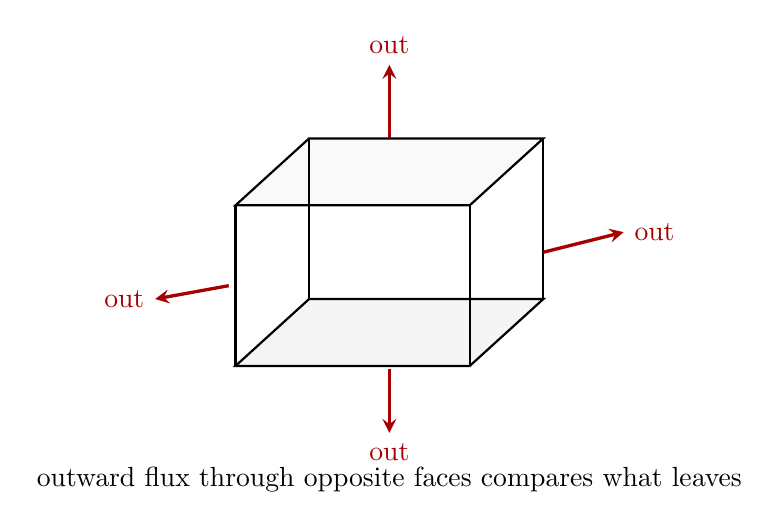
\begin{tikzpicture}[scale=0.85, >=stealth]
    \coordinate (O) at (0,0);
    \coordinate (A) at (3.5,0);
    \coordinate (B) at (4.6,1.0);
    \coordinate (C) at (1.1,1.0);
    \coordinate (D) at (0,2.4);
    \coordinate (E) at (3.5,2.4);
    \coordinate (F) at (4.6,3.4);
    \coordinate (G) at (1.1,3.4);

    \draw[fill=gray!8, thick] (O)--(A)--(B)--(C)--cycle;
    \draw[fill=gray!5, thick] (D)--(E)--(F)--(G)--cycle;
    \draw[thick] (O)--(D);
    \draw[thick] (A)--(E);
    \draw[thick] (B)--(F);
    \draw[thick] (C)--(G);

    \draw[->, very thick, red!65!black] (4.6,1.7) -- (5.8,2.0)
        node[right] {out};
    \draw[->, very thick, red!65!black] (-0.1,1.2) -- (-1.2,1.0)
        node[left] {out};
    \draw[->, very thick, red!65!black] (2.3,3.4) -- (2.3,4.5)
        node[above] {out};
    \draw[->, very thick, red!65!black] (2.3,-0.05) -- (2.3,-1.0)
        node[below] {out};

    \node at (2.3,-1.7) {outward flux through opposite faces compares what leaves};
\end{tikzpicture}
\caption{Divergence measures net outward flux per unit volume.}
\end{figure}

\subsection{Divergence as source density}

For a general field
\[
    \mathbf F=(P,Q,R),
\]
the same small-box argument gives
\[
\boxed{
    \text{net outward flux through a tiny box}
    \approx
    (P_x+Q_y+R_z)\,\Delta V.
}
\]
The coefficient gets its own name.

\begin{definition}[Divergence]
Let
\[
    \mathbf F=(P,Q,R)
\]
be a vector field in space.  The \emph{divergence} of \(\mathbf F\) is
\[
\boxed{
    \nabla\cdot\mathbf F
    =
    P_x+Q_y+R_z.
}
\]
\end{definition}

If
\[
    \nabla\cdot\mathbf F>0,
\]
then the field has net outward flow from a small box.  It behaves like a source.

If
\[
    \nabla\cdot\mathbf F<0,
\]
then more flow enters a small box than leaves.  It behaves like a sink.

If
\[
    \nabla\cdot\mathbf F=0,
\]
then there is no net creation or loss at that point.  Fluid may still move, swirl, and
bend, but it is not locally expanding or compressing.

\begin{example}[A swirling field has zero divergence]
Let
\[
    \mathbf F(x,y,z)=(-y,x,0).
\]
Then
\[
    P=-y,\qquad Q=x,\qquad R=0.
\]
So
\[
    \nabla\cdot\mathbf F
    =
    P_x+Q_y+R_z
    =
    0+0+0
    =
    0.
\]
This field rotates around the \(z\)-axis, but it does not create net outward flow from
small boxes.
\end{example}

\begin{example}[A radial field has positive divergence]
Let
\[
    \mathbf F(x,y,z)=(x,y,z).
\]
Then
\[
    \nabla\cdot\mathbf F=1+1+1=3.
\]
Every small box has net outward flux approximately
\[
    3\,\Delta V.
\]
The field points away from the origin and expands space uniformly.
\end{example}

\subsection{Divergence in form language}

The flux \(2\)-form of
\[
    \mathbf F=(P,Q,R)
\]
is
\[
    \Phi_{\mathbf F}
    =
    P\,dy\wedge dz
    +
    Q\,dz\wedge dx
    +
    R\,dx\wedge dy.
\]
Take its exterior derivative:
\[
\begin{aligned}
d\Phi_{\mathbf F}
&=
dP\wedge dy\wedge dz
+
dQ\wedge dz\wedge dx
+
dR\wedge dx\wedge dy.
\end{aligned}
\]
Only one term from each differential survives:
\[
    dP\wedge dy\wedge dz
    =
    P_x\,dx\wedge dy\wedge dz,
\]
\[
    dQ\wedge dz\wedge dx
    =
    Q_y\,dy\wedge dz\wedge dx
    =
    Q_y\,dx\wedge dy\wedge dz,
\]
and
\[
    dR\wedge dx\wedge dy
    =
    R_z\,dz\wedge dx\wedge dy
    =
    R_z\,dx\wedge dy\wedge dz.
\]
Therefore
\[
\boxed{
    d\Phi_{\mathbf F}
    =
    (P_x+Q_y+R_z)\,dx\wedge dy\wedge dz.
}
\]
So
\[
\boxed{
    d\Phi_{\mathbf F}
    =
    (\nabla\cdot\mathbf F)\,dx\wedge dy\wedge dz.
}
\]

This is the next piece of the pattern:

\[
\begin{array}{c|c|c}
\text{object} & \text{exterior derivative} & \text{classical name}\\ \hline
f & df & \text{gradient information}\\[1mm]
P\,dx+Q\,dy+R\,dz & d\omega & \text{curl flux form}\\[1mm]
P\,dy\wedge dz+Q\,dz\wedge dx+R\,dx\wedge dy & d\Phi & \text{divergence volume form}
\end{array}
\]

The derivative of a \(2\)-form is a \(3\)-form.  Flux through a surface becomes source
density inside a solid.

\subsection{The divergence theorem}

Now tile a solid region by many small boxes.  On each small box,
\[
    \text{outward flux}
    \approx
    (\nabla\cdot\mathbf F)\Delta V.
\]
Add all boxes.

On the left side, flux across interior faces cancels.  One small box sees the shared face
as outward, while the neighboring box sees the same face with the opposite normal.
The two contributions have opposite signs.

Only the outer boundary remains.

On the right side, the sums become a triple integral:
\[
    \sum(\nabla\cdot\mathbf F)\Delta V
    \longrightarrow
    \iiint_E \nabla\cdot\mathbf F\,dV.
\]

This gives the divergence theorem.

\begin{theorem}[Divergence theorem]
Let \(E\) be a solid region in space with piecewise smooth closed boundary
\[
    \partial E.
\]
Give \(\partial E\) the outward orientation.  Let
\[
    \mathbf F=(P,Q,R)
\]
have continuous first partial derivatives on an open region containing \(E\).  Then
\[
\boxed{
    \iint_{\partial E}
    \mathbf F\cdot\widehat{\mathbf n}\,dS
    =
    \iiint_E
    \nabla\cdot\mathbf F\,dV.
}
\]
In differential-form notation,
\[
\boxed{
    \int_{\partial E}\Phi_{\mathbf F}
    =
    \int_E d\Phi_{\mathbf F}.
}
\]
\end{theorem}

The theorem says:

\[
\boxed{
    \text{net outward flux through the boundary}
    =
    \text{total source strength inside}.
}
\]

This is the three-dimensional cousin of Green's theorem and Stokes' theorem.  Once
again, an integral over a boundary equals an integral of a derivative over the inside.

\subsection{Outward flux through a sphere}

Let \(S\) be the sphere of radius \(a\) centered at the origin, with outward orientation.
Let
\[
    \mathbf F(x,y,z)=(x,y,z).
\]
In Section \ref{sec:15.3}, we computed this flux directly and found
\[
    4\pi a^3.
\]
Now the divergence theorem gives it almost immediately.

Let \(E\) be the ball
\[
    x^2+y^2+z^2\le a^2.
\]
The divergence is
\[
    \nabla\cdot\mathbf F=3.
\]
Therefore
\[
\begin{aligned}
\iint_S \mathbf F\cdot\widehat{\mathbf n}\,dS
&=
\iiint_E 3\,dV\\
&=
3\operatorname{Volume}(E)\\
&=
3\left(\frac43\pi a^3\right)\\
&=
4\pi a^3.
\end{aligned}
\]
So
\[
\boxed{
    \iint_S (x,y,z)\cdot\widehat{\mathbf n}\,dS=4\pi a^3.
}
\]
The surface calculation became a volume calculation.

\subsection{A closed cylinder}

Let \(E\) be the solid cylinder
\[
    x^2+y^2\le a^2,
    \qquad
    0\le z\le h.
\]
Its boundary has three pieces:

\[
\begin{array}{c|c}
\text{piece} & \text{description}\\ \hline
S_{\text{side}} & x^2+y^2=a^2,\quad 0\le z\le h\\[1mm]
S_{\text{top}} & x^2+y^2\le a^2,\quad z=h\\[1mm]
S_{\text{bottom}} & x^2+y^2\le a^2,\quad z=0
\end{array}
\]

Use
\[
    \mathbf F=(x,y,z).
\]
Again
\[
    \nabla\cdot\mathbf F=3.
\]
So the total outward flux through the closed cylinder is
\[
\begin{aligned}
\iint_{\partial E}\mathbf F\cdot\widehat{\mathbf n}\,dS
&=
\iiint_E 3\,dV\\
&=
3\pi a^2h.
\end{aligned}
\]
Thus
\[
\boxed{
    \text{total outward flux}=3\pi a^2h.
}
\]

We can see the pieces too.

On the side, Section \ref{sec:15.3} showed that for
\[
    (x,y,0)
\]
the outward side flux is
\[
    2\pi a^2h.
\]
The \(z\)-component is tangent to the side, so the same side flux holds for
\[
    (x,y,z).
\]

On the top,
\[
    \widehat{\mathbf n}=(0,0,1),
\]
so
\[
    \mathbf F\cdot\widehat{\mathbf n}=h.
\]
The top area is
\[
    \pi a^2,
\]
so the top flux is
\[
    h\pi a^2.
\]

On the bottom,
\[
    \widehat{\mathbf n}=(0,0,-1),
\]
but
\[
    z=0,
\]
so
\[
    \mathbf F\cdot\widehat{\mathbf n}=0.
\]
The bottom flux is \(0\).

Adding:
\[
    2\pi a^2h+\pi a^2h+0=3\pi a^2h.
\]
The divergence theorem found the total at once.

\subsection{Using symmetry: a paraboloid cap}

The divergence theorem is especially helpful when a surface integral would be awkward.

Let \(S\) be the curved paraboloid
\[
    z=4-x^2-y^2,
    \qquad
    x^2+y^2\le4,
\]
oriented upward.  Together with the disk
\[
    D:\quad z=0,\qquad x^2+y^2\le4,
\]
it bounds a solid region \(E\).

Let
\[
    \mathbf F=(0,0,z).
\]
We want the flux through the curved paraboloid \(S\).

The divergence is
\[
    \nabla\cdot\mathbf F=1.
\]
So the total outward flux through the closed surface
\[
    S\cup D
\]
is
\[
    \iiint_E 1\,dV=\operatorname{Volume}(E).
\]
The volume is
\[
\begin{aligned}
\operatorname{Volume}(E)
&=
\int_0^{2\pi}\int_0^2(4-r^2)r\,dr\,d\theta\\
&=
2\pi\left[2r^2-\frac{r^4}{4}\right]_0^2\\
&=
2\pi(8-4)\\
&=
8\pi.
\end{aligned}
\]
On the bottom disk, \(z=0\), so
\[
    \mathbf F=(0,0,0).
\]
The bottom flux is \(0\).  Therefore the flux through the curved paraboloid is
\[
\boxed{
    8\pi.
}
\]
The theorem let the solid volume do the work.

\subsection{Why the hypotheses matter}

The divergence theorem has three common traps: the surface must be closed, the normal
must point outward, and the field must be defined throughout the solid.

\subsubsection*{A single open surface is not enough}

Let \(D\) be the disk
\[
    x^2+y^2\le1,\qquad z=0,
\]
oriented upward.  Let
\[
    \mathbf F=(0,0,1).
\]
The flux through the disk is
\[
    \iint_D 1\,dS=\pi.
\]
But
\[
    \nabla\cdot\mathbf F=0.
\]

This does not contradict the divergence theorem.  The disk alone is not a closed
surface.  It is not the entire boundary of a solid.  To use the theorem, we would need a
closed surface, such as the boundary of a cylinder or a half-ball.

\subsubsection*{Outward orientation matters}

Take the unit cube
\[
    E=[0,1]\times[0,1]\times[0,1]
\]
and the field
\[
    \mathbf F=(x,0,0).
\]
The divergence is
\[
    \nabla\cdot\mathbf F=1.
\]
So the divergence theorem predicts outward flux
\[
    \iiint_E 1\,dV=1.
\]

Indeed, only the two \(x\)-faces contribute.  On \(x=1\), the outward normal is
\(\mathbf i\), and the flux is \(1\).  On \(x=0\), the field is zero.  Total outward flux:
\[
    1.
\]

If we choose inward normals instead, every sign reverses and the flux is
\[
    -1.
\]
The theorem uses outward orientation.

\subsubsection*{The field must be defined inside}

Consider the inverse-square radial field
\[
    \mathbf G(x,y,z)
    =
    \frac{(x,y,z)}{(x^2+y^2+z^2)^{3/2}}.
\]
This field is not defined at the origin.

Away from the origin, write
\[
    r=\sqrt{x^2+y^2+z^2}.
\]
Then
\[
    \mathbf G=\left(\frac{x}{r^3},\frac{y}{r^3},\frac{z}{r^3}\right).
\]
A direct calculation gives, for \(r>0\),
\[
\begin{aligned}
\nabla\cdot\mathbf G
&=
\left(r^{-3}-3x^2r^{-5}\right)
+
\left(r^{-3}-3y^2r^{-5}\right)
+
\left(r^{-3}-3z^2r^{-5}\right)\\
&=
3r^{-3}-3(x^2+y^2+z^2)r^{-5}\\
&=
3r^{-3}-3r^2r^{-5}\\
&=
0.
\end{aligned}
\]

Now take the sphere \(S_a\) of radius \(a\), oriented outward.  On this sphere,
\[
    \widehat{\mathbf n}=\frac{(x,y,z)}{a},
\]
and
\[
    \mathbf G=\frac{(x,y,z)}{a^3}.
\]
Thus
\[
\begin{aligned}
\mathbf G\cdot\widehat{\mathbf n}
&=
\frac{(x,y,z)}{a^3}\cdot \frac{(x,y,z)}{a}\\
&=
\frac{x^2+y^2+z^2}{a^4}\\
&=
\frac{a^2}{a^4}\\
&=
\frac1{a^2}.
\end{aligned}
\]
Therefore
\[
\begin{aligned}
\iint_{S_a}\mathbf G\cdot\widehat{\mathbf n}\,dS
&=
\frac1{a^2}\cdot 4\pi a^2\\
&=
4\pi.
\end{aligned}
\]

It would be wrong to say:
\[
    \nabla\cdot\mathbf G=0,
    \qquad
    \text{so the flux through the sphere is }0.
\]
The field is not defined at the origin, and the origin lies inside the sphere.  The
divergence theorem cannot be applied to the whole ball.

If we remove the singularity, the theorem works again.  Let \(E\) be the spherical shell
\[
    b\le r\le a,
    \qquad 0<b<a.
\]
On this shell,
\[
    \nabla\cdot\mathbf G=0.
\]
The boundary has two pieces.  The outer sphere contributes
\[
    4\pi.
\]
On the inner sphere \(r=b\), the outward normal for the shell points toward the center,
so it is
\[
    -\widehat{\mathbf r}.
\]
The inner flux is
\[
    -4\pi.
\]
The total flux is
\[
    4\pi-4\pi=0,
\]
which matches
\[
    \iiint_E 0\,dV=0.
\]

The missing point was carrying the source.

\subsection{Physical meaning: conservation and balance}

If \(\mathbf F\) is a velocity field of a fluid, then
\[
    \mathbf F\cdot\widehat{\mathbf n}
\]
measures flow rate through a unit area.  The flux through a closed surface measures
net flow leaving the region.

The divergence theorem says that this net outflow can be computed by adding local
source strengths:
\[
    \iint_{\partial E}\mathbf F\cdot\widehat{\mathbf n}\,dS
    =
    \iiint_E \nabla\cdot\mathbf F\,dV.
\]

If
\[
    \nabla\cdot\mathbf F=0
\]
throughout \(E\), then
\[
    \iint_{\partial E}\mathbf F\cdot\widehat{\mathbf n}\,dS=0.
\]
Fluid may pass through the region, but whatever enters also leaves.  There is no net
creation inside.

If
\[
    \nabla\cdot\mathbf F>0
\]
on average, more fluid leaves than enters.  Something inside acts like a source.

If
\[
    \nabla\cdot\mathbf F<0
\]
on average, more fluid enters than leaves.  Something inside acts like a sink.

This is the mathematical language behind conservation laws.  To know how much
quantity changes inside a region, look at what crosses the boundary and what is
created or destroyed inside.

We now have two space derivatives of vector fields:
\[
    \nabla\times\mathbf F
    \qquad\text{and}\qquad
    \nabla\cdot\mathbf F.
\]
One measures spinning; the other measures spreading.  They look unrelated in vector
notation.  But in form notation they are consecutive exterior derivatives:
\[
    \omega
    \xrightarrow{\ d\ }
    d\omega
    \xrightarrow{\ d\ }
    d(d\omega).
\]
That raises a strange question.  What happens if we take \(d\) twice?  The answer is
always zero, and it hides two famous vector-calculus identities:
\[
    \nabla\times(\nabla f)=\mathbf 0,
    \qquad
    \nabla\cdot(\nabla\times\mathbf F)=0.
\]
The next section explains why these are not two miracles.  They are one fact wearing
two costumes.
\section{Classical vector-calculus identities}
\label{sec:15.7}

Section \ref{sec:15.6} ended with two familiar-looking derivatives:
\[
    \nabla\times \mathbf F
    \qquad\text{and}\qquad
    \nabla\cdot \mathbf F.
\]
In vector notation they look like separate operations.  In form notation they are
successive appearances of the same operation:
\[
    d.
\]
That is why two famous identities are really one fact.

\subsection{A gradient field has no local rotation}

Suppose a metal plate has temperature
\[
    T(x,y,z)=x^2y+yz+3z.
\]
The gradient field is
\[
    \nabla T=(2xy,\ x^2+z,\ y+3).
\]
This field points in the direction of fastest temperature increase.

Compute its curl:
\[
\begin{aligned}
\nabla\times(\nabla T)
&=
\left(
\frac{\partial}{\partial y}(y+3)
-
\frac{\partial}{\partial z}(x^2+z),
\right.\\
&\qquad
\frac{\partial}{\partial z}(2xy)
-
\frac{\partial}{\partial x}(y+3),
\\
&\qquad\left.
\frac{\partial}{\partial x}(x^2+z)
-
\frac{\partial}{\partial y}(2xy)
\right)\\[1mm]
&=
(1-1,\ 0-0,\ 2x-2x)\\
&=
\mathbf 0.
\end{aligned}
\]

The cancellations are not an accident.  A gradient field comes from a potential
function.  It points uphill.  A tiny paddle wheel placed in a pure uphill field may be
pushed, but it has no first-order tendency to spin.

In the language of \(1\)-forms, the potential \(T\) has differential
\[
    dT=T_x\,dx+T_y\,dy+T_z\,dz.
\]
For our example,
\[
    dT=2xy\,dx+(x^2+z)\,dy+(y+3)\,dz.
\]
Taking \(d\) again gives
\[
    d(dT)=0.
\]
That is the form version of
\[
    \nabla\times(\nabla T)=\mathbf 0.
\]

\begin{theorem}[Curl of a gradient]
Let \(f(x,y,z)\) have continuous second partial derivatives on an open region.  Then
\[
\boxed{
    \nabla\times(\nabla f)=\mathbf 0.
}
\]
Equivalently,
\[
\boxed{
    d(df)=0.
}
\]
\end{theorem}

\begin{proof}
Write
\[
    \nabla f=(f_x,f_y,f_z).
\]
Then
\[
\begin{aligned}
\nabla\times(\nabla f)
&=
(f_{zy}-f_{yz},\ f_{xz}-f_{zx},\ f_{yx}-f_{xy}).
\end{aligned}
\]
If the second partial derivatives are continuous, then the mixed partials agree:
\[
    f_{zy}=f_{yz},\qquad
    f_{xz}=f_{zx},\qquad
    f_{yx}=f_{xy}.
\]
So every component is zero.
\end{proof}

The hypothesis about continuous second partial derivatives is doing real work.

\begin{example}[Why the smoothness hypothesis matters]
Define
\[
    f(x,y)=
    \begin{cases}
    \dfrac{xy(x^2-y^2)}{x^2+y^2}, & (x,y)\ne(0,0),\\[2mm]
    0, & (x,y)=(0,0).
    \end{cases}
\]
This function has second mixed partial derivatives at the origin, but they are not equal.

First compute \(f_x(0,y)\).  For \(y\ne0\),
\[
\begin{aligned}
f_x(0,y)
&=
\lim_{h\to0}
\frac{f(h,y)-f(0,y)}{h}\\
&=
\lim_{h\to0}
\frac{hy(h^2-y^2)}{h^2+y^2}\cdot\frac1h\\
&=
\lim_{h\to0}
y\frac{h^2-y^2}{h^2+y^2}\\
&=
-y.
\end{aligned}
\]
Also \(f_x(0,0)=0\).  Therefore
\[
    f_{xy}(0,0)
    =
    \lim_{y\to0}\frac{f_x(0,y)-f_x(0,0)}{y}
    =
    \lim_{y\to0}\frac{-y}{y}
    =
    -1.
\]

Now compute \(f_y(x,0)\).  For \(x\ne0\),
\[
\begin{aligned}
f_y(x,0)
&=
\lim_{h\to0}
\frac{f(x,h)-f(x,0)}{h}\\
&=
\lim_{h\to0}
\frac{xh(x^2-h^2)}{x^2+h^2}\cdot\frac1h\\
&=
\lim_{h\to0}
x\frac{x^2-h^2}{x^2+h^2}\\
&=
x.
\end{aligned}
\]
Also \(f_y(0,0)=0\).  Therefore
\[
    f_{yx}(0,0)
    =
    \lim_{x\to0}\frac{f_y(x,0)-f_y(0,0)}{x}
    =
    \lim_{x\to0}\frac{x}{x}
    =
    1.
\]

So
\[
\boxed{
    f_{xy}(0,0)=-1,
    \qquad
    f_{yx}(0,0)=1.
}
\]
If we form the field
\[
    \nabla f=(f_x,f_y,0),
\]
then at the origin the \(z\)-component of
\[
    \nabla\times(\nabla f)
\]
would be
\[
    f_{yx}(0,0)-f_{xy}(0,0)=2.
\]
The identity failed because the second partial derivatives were not continuous enough
to force mixed partials to agree.
\end{example}

The moral is small but sharp: the identity
\[
    \nabla\times(\nabla f)=\mathbf 0
\]
belongs to sufficiently smooth functions.  It is not a purely formal trick with symbols.

\subsection{A curl field has no source strength}

Now look at a curl instead of a gradient.

Let
\[
    \mathbf F(x,y,z)=(0,xz,0).
\]
Then
\[
\begin{aligned}
\nabla\times\mathbf F
&=
\left(
0-\frac{\partial}{\partial z}(xz),
\frac{\partial}{\partial z}(0)-0,
\frac{\partial}{\partial x}(xz)-0
\right)\\
&=
(-x,0,z).
\end{aligned}
\]
Now take its divergence:
\[
\begin{aligned}
\nabla\cdot(\nabla\times\mathbf F)
&=
\frac{\partial}{\partial x}(-x)
+
\frac{\partial}{\partial y}(0)
+
\frac{\partial}{\partial z}(z)\\
&=
-1+0+1\\
&=
0.
\end{aligned}
\]

A curl field represents local spinning.  Spinning can move material around, but by
itself it does not create source strength.  In form language, if
\[
    \omega=P\,dx+Q\,dy+R\,dz
\]
is the work form of \(\mathbf F\), then
\[
    d\omega
\]
is the flux form of \(\nabla\times\mathbf F\).  Taking \(d\) again gives
\[
    d(d\omega)=0.
\]
That is the form version of
\[
    \nabla\cdot(\nabla\times\mathbf F)=0.
\]

\begin{theorem}[Divergence of a curl]
Let
\[
    \mathbf F=(P,Q,R)
\]
have continuous second partial derivatives on an open region.  Then
\[
\boxed{
    \nabla\cdot(\nabla\times\mathbf F)=0.
}
\]
Equivalently, if
\[
    \omega=P\,dx+Q\,dy+R\,dz,
\]
then
\[
\boxed{
    d(d\omega)=0.
}
\]
\end{theorem}

\begin{proof}
The curl is
\[
    \nabla\times\mathbf F
    =
    (R_y-Q_z,\ P_z-R_x,\ Q_x-P_y).
\]
Its divergence is
\[
\begin{aligned}
\nabla\cdot(\nabla\times\mathbf F)
&=
(R_y-Q_z)_x
+
(P_z-R_x)_y
+
(Q_x-P_y)_z\\
&=
R_{yx}-Q_{zx}+P_{zy}-R_{xy}+Q_{xz}-P_{yz}.
\end{aligned}
\]
Regroup:
\[
    (R_{yx}-R_{xy})
    +
    (P_{zy}-P_{yz})
    +
    (Q_{xz}-Q_{zx}).
\]
Each pair cancels because the second partial derivatives are continuous.  Therefore
\[
    \nabla\cdot(\nabla\times\mathbf F)=0.
\]
\end{proof}

The same smoothness warning appears again.

\begin{example}[A nonsmooth vector potential can break the cancellation]
Use the function from the previous example:
\[
    f(x,y)=
    \begin{cases}
    \dfrac{xy(x^2-y^2)}{x^2+y^2}, & (x,y)\ne(0,0),\\[2mm]
    0, & (x,y)=(0,0).
    \end{cases}
\]
Define a vector field in space by
\[
    \mathbf A(x,y,z)=(0,0,f(x,y)).
\]
Then
\[
    \nabla\times\mathbf A=(f_y,-f_x,0).
\]
At the origin,
\[
\begin{aligned}
\nabla\cdot(\nabla\times\mathbf A)
&=
(f_y)_x+(-f_x)_y\\
&=
f_{yx}-f_{xy}\\
&=
1-(-1)\\
&=
2.
\end{aligned}
\]
So the identity
\[
    \nabla\cdot(\nabla\times\mathbf A)=0
\]
fails at the origin.  The formal cancellation depends on the mixed partials being
allowed to trade order.
\end{example}

\subsection{The single fact: \texorpdfstring{\(d^2=0\)}{d squared is zero}}

The two identities now have the same explanation.

For a function \(f\),
\[
    df
\]
is a \(1\)-form.  Its exterior derivative is
\[
    d(df).
\]
The identity
\[
    d(df)=0
\]
is the statement
\[
    \nabla\times(\nabla f)=\mathbf 0.
\]

For a work \(1\)-form
\[
    \omega=P\,dx+Q\,dy+R\,dz,
\]
the derivative
\[
    d\omega
\]
is the flux \(2\)-form of the curl:
\[
    d\omega=\Phi_{\nabla\times\mathbf F}.
\]
The identity
\[
    d(d\omega)=0
\]
is the statement
\[
    \nabla\cdot(\nabla\times\mathbf F)=0.
\]

So the two classical identities are one rule:
\[
\boxed{
    d^2=0.
}
\]

A tiny piece of the algebra shows why.  In two variables,
\[
    df=f_x\,dx+f_y\,dy.
\]
Then
\[
\begin{aligned}
d(df)
&=
d(f_x)\wedge dx+d(f_y)\wedge dy\\
&=
(f_{xx}\,dx+f_{xy}\,dy)\wedge dx
+
(f_{yx}\,dx+f_{yy}\,dy)\wedge dy.
\end{aligned}
\]
Now
\[
    dx\wedge dx=0,
    \qquad
    dy\wedge dy=0,
\]
and
\[
    dy\wedge dx=-dx\wedge dy.
\]
So
\[
\begin{aligned}
d(df)
&=
f_{xy}\,dy\wedge dx+f_{yx}\,dx\wedge dy\\
&=
(f_{yx}-f_{xy})\,dx\wedge dy.
\end{aligned}
\]
When the mixed partials agree, this is \(0\).

The wedge product supplies the sign.  Equality of mixed partials supplies the
cancellation.

\subsection{Potentials and topology warnings}

The identity
\[
    \nabla\times(\nabla f)=\mathbf 0
\]
says every gradient field has zero curl.

The converse is more delicate.  If
\[
    \nabla\times\mathbf F=\mathbf 0,
\]
then \(\mathbf F\) often has a potential function locally.  On a simple region with no
holes, it may have a global potential:
\[
    \mathbf F=\nabla f.
\]
But holes can prevent a global potential.

Recall the field
\[
    \mathbf A(x,y,z)
    =
    \left(
    -\frac{y}{x^2+y^2},
    \frac{x}{x^2+y^2},
    0
    \right),
\]
defined away from the \(z\)-axis.  A direct calculation gives
\[
    \nabla\times\mathbf A=\mathbf 0
\]
where the field is defined.

But around the unit circle
\[
    \mathbf r(t)=(\cos t,\sin t,0),
    \qquad 0\le t\le2\pi,
\]
we get
\[
    \mathbf A(\mathbf r(t))=(-\sin t,\cos t,0),
\]
and
\[
    \mathbf r'(t)=(-\sin t,\cos t,0).
\]
Thus
\[
\begin{aligned}
\oint_C \mathbf A\cdot d\mathbf r
&=
\int_0^{2\pi}
(-\sin t,\cos t,0)\cdot(-\sin t,\cos t,0)\,dt\\
&=
\int_0^{2\pi}1\,dt\\
&=
2\pi.
\end{aligned}
\]
If \(\mathbf A\) were a global gradient field on its whole domain, every closed-loop
integral would be \(0\).  This nonzero integral proves that no such global potential
exists.

A similar warning appears one level higher.  The identity
\[
    \nabla\cdot(\nabla\times\mathbf A)=0
\]
says every curl field has zero divergence.  The converse asks whether every
divergence-free field can be written as a curl:
\[
    \mathbf F=\nabla\times\mathbf A.
\]
Again, topology can interfere.

Consider
\[
    \mathbf G(x,y,z)
    =
    \frac{(x,y,z)}{(x^2+y^2+z^2)^{3/2}},
\]
defined on
\[
    \mathbb R^3\setminus\{(0,0,0)\}.
\]
Away from the origin,
\[
    \nabla\cdot\mathbf G=0.
\]
But the outward flux through any sphere centered at the origin is
\[
    4\pi.
\]
If \(\mathbf G=\nabla\times\mathbf A\) for a smooth vector field \(\mathbf A\) defined
on the punctured space, then the flux of \(\mathbf G\) through the sphere would be the
flux of a curl through a closed surface.  Stokes' theorem would give
\[
    \iint_S(\nabla\times\mathbf A)\cdot\widehat{\mathbf n}\,dS
    =
    \int_{\partial S}\mathbf A\cdot d\mathbf r
    =
    0,
\]
because a sphere has no boundary.  But the flux is \(4\pi\).  So no global vector
potential exists on the punctured space.

These warnings are not exceptions to the identities.  They say something more subtle:
local derivative tests do not always decide global questions.  Smoothness and domain
shape both matter.

That is why the final section of the chapter collects the traps.  The formulas are short,
but the surface, the orientation, the boundary, and the domain decide whether the
formula may be used.

\section{Warning examples}
\label{sec:15.8}

The three big theorems in this chapter are easy to state:
\[
    \int_{\partial S}\omega=\int_S d\omega,
    \qquad
    \int_{\partial E}\Phi=\int_E d\Phi.
\]
Their hypotheses are where many mistakes happen.  A surface may have no consistent
normal direction.  A field may be undefined at one hidden point.  A boundary may be
walked the wrong way.  A region may have an inner boundary that should not be
ignored.

Each warning below is a small failure of one of those hidden assumptions.

\subsection{A nonorientable surface and why flux is not globally defined}

A flux integral needs a chosen side:
\[
    \iint_S \mathbf F\cdot\widehat{\mathbf n}\,dS.
\]
That means \(S\) must have a continuous unit normal vector field
\[
    \widehat{\mathbf n}
\]
on the whole surface.

A sphere has two sides, inside and outside.  A cylinder has two sides, inside and
outside.  A disk has two sides, up and down.

A M\"obius strip does not.

One parametrization of a M\"obius strip is
\[
\mathbf r(u,v)=
\left(
\left(2+v\cos\frac u2\right)\cos u,\,
\left(2+v\cos\frac u2\right)\sin u,\,
v\sin\frac u2
\right),
\]
where
\[
    0\le u\le2\pi,
    \qquad
    -\frac12\le v\le \frac12.
\]
The point at \(u=0\) with parameter \(v\) is identified with the point at \(u=2\pi\)
with parameter \(-v\).  That twist is the whole issue.

If you choose a normal vector at one point and slide it continuously around the center
of the strip, it returns to the same physical point pointing the opposite way.  The
surface has only one side.

\begin{figure}[h]
\centering
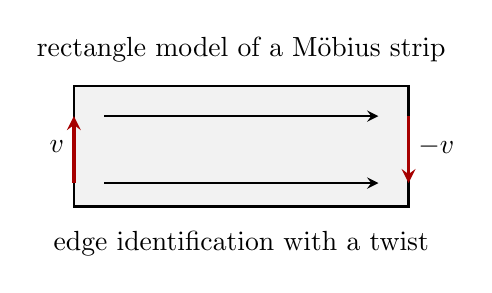
\begin{tikzpicture}[scale=0.85, >=stealth]
    \draw[thick, fill=gray!10] (0,0) rectangle (5,1.8);

    \draw[->, very thick, red!65!black] (0,0.35) -- (0,1.35);
    \draw[->, very thick, red!65!black] (5,1.35) -- (5,0.35);

    \node[left] at (0,0.9) {\(v\)};
    \node[right] at (5,0.9) {\(-v\)};

    \draw[->, thick] (0.45,1.35) -- (4.55,1.35);
    \draw[->, thick] (0.45,0.35) -- (4.55,0.35);

    \node at (2.5,-0.55) {edge identification with a twist};
    \node at (2.5,2.35) {rectangle model of a M\"obius strip};
\end{tikzpicture}
\caption{The M\"obius strip is made by identifying opposite ends with a twist.  A normal
direction reverses after one trip around the strip.}
\end{figure}

A scalar surface integral still makes sense:
\[
    \iint_S f\,dS.
\]
Area has no sign, so it does not need a side.

But flux is signed.  It asks whether the field crosses the positive side or the negative
side.  On a M\"obius strip there is no globally consistent positive side.  So a global
flux integral
\[
    \iint_S \mathbf F\cdot\widehat{\mathbf n}\,dS
\]
is not defined.

The problem is not the vector field.  The problem is the surface.

\subsection{A field with nonzero flux because of a hidden singularity}

The divergence theorem says
\[
    \iint_{\partial E}\mathbf F\cdot\widehat{\mathbf n}\,dS
    =
    \iiint_E \nabla\cdot\mathbf F\,dV.
\]
But the field must be defined and differentiable throughout the solid \(E\), not only
on its boundary.

Consider again
\[
    \mathbf G(x,y,z)
    =
    \frac{(x,y,z)}{(x^2+y^2+z^2)^{3/2}}.
\]
Away from the origin,
\[
    \nabla\cdot\mathbf G=0.
\]
Now take the sphere \(S_a\) of radius \(a\), oriented outward.  On the sphere,
\[
    \widehat{\mathbf n}=\frac{(x,y,z)}{a},
\]
and
\[
    \mathbf G=\frac{(x,y,z)}{a^3}.
\]
Therefore
\[
\begin{aligned}
\mathbf G\cdot\widehat{\mathbf n}
&=
\frac{(x,y,z)}{a^3}\cdot\frac{(x,y,z)}{a}\\
&=
\frac{x^2+y^2+z^2}{a^4}\\
&=
\frac{a^2}{a^4}\\
&=
\frac1{a^2}.
\end{aligned}
\]
Thus
\[
\begin{aligned}
\iint_{S_a}\mathbf G\cdot\widehat{\mathbf n}\,dS
&=
\frac1{a^2}\cdot 4\pi a^2\\
&=
4\pi.
\end{aligned}
\]

It would be tempting to say:
\[
    \nabla\cdot\mathbf G=0,
    \qquad
    \text{so the flux should be }0.
\]
That is not allowed.  The origin is inside the sphere, and the field is not defined
there.

The missing point behaves like a source.  The divergence calculation sees zero
everywhere it is allowed to look, but the flux through the sphere reveals that something
has been hidden inside.

\subsection{Stokes' theorem with incompatible orientations}

Stokes' theorem needs the orientation of the surface and the orientation of its boundary
to match.

Let
\[
    \mathbf F(x,y,z)=\left(-\frac y2,\frac x2,0\right).
\]
Then
\[
    \nabla\times\mathbf F=(0,0,1).
\]
Let \(D\) be the unit disk in the plane \(z=0\), oriented upward.  Then
\[
\begin{aligned}
\iint_D(\nabla\times\mathbf F)\cdot\widehat{\mathbf n}\,dS
&=
\iint_D(0,0,1)\cdot(0,0,1)\,dS\\
&=
\pi.
\end{aligned}
\]

The upward orientation gives the boundary circle the counterclockwise orientation as
seen from above.  With that direction,
\[
    \oint_{\partial D}\mathbf F\cdot d\mathbf r=\pi.
\]

But now walk around the same circle clockwise.  A convenient parametrization is
\[
    \mathbf r(t)=(\cos t,-\sin t,0),
    \qquad 0\le t\le2\pi.
\]
Then
\[
    \mathbf r'(t)=(-\sin t,-\cos t,0),
\]
and
\[
    \mathbf F(\mathbf r(t))
    =
    \left(\frac{\sin t}{2},\frac{\cos t}{2},0\right).
\]
So
\[
\begin{aligned}
\oint_C\mathbf F\cdot d\mathbf r
&=
\int_0^{2\pi}
\left(\frac{\sin t}{2},\frac{\cos t}{2},0\right)
\cdot
(-\sin t,-\cos t,0)
\,dt\\
&=
-\frac12\int_0^{2\pi}1\,dt\\
&=
-\pi.
\end{aligned}
\]

The line integral is now
\[
    -\pi,
\]
but the upward surface integral is still
\[
    \pi.
\]
There is no contradiction.  The clockwise boundary is not compatible with the upward
normal.  It would be compatible with the downward normal.

The theorem did not fail.  The orientation choice failed.

\subsection{The divergence theorem on a region with an inner boundary}

A region with a hole has more than one boundary piece.  The divergence theorem counts
all of them.

Let \(E\) be the spherical shell
\[
    b\le r\le a,
    \qquad
    0<b<a,
\]
where
\[
    r=\sqrt{x^2+y^2+z^2}.
\]
Its boundary has two pieces:
\[
    S_a:\ r=a,
    \qquad
    S_b:\ r=b.
\]
The outward normal on the outer sphere \(S_a\) points away from the origin.  The
outward normal on the inner sphere \(S_b\), for the shell, points toward the origin.

Take the field
\[
    \mathbf F(x,y,z)=(x,y,z).
\]
Then
\[
    \nabla\cdot\mathbf F=3.
\]
The divergence theorem gives
\[
\begin{aligned}
\iint_{\partial E}\mathbf F\cdot\widehat{\mathbf n}\,dS
&=
\iiint_E 3\,dV\\
&=
3\left(\frac43\pi a^3-\frac43\pi b^3\right)\\
&=
4\pi(a^3-b^3).
\end{aligned}
\]

Now check the boundary pieces.

On \(S_a\),
\[
    \widehat{\mathbf n}=\frac{(x,y,z)}{a},
\]
so
\[
    \mathbf F\cdot\widehat{\mathbf n}=a.
\]
Thus
\[
    \iint_{S_a}\mathbf F\cdot\widehat{\mathbf n}\,dS
    =
    a\cdot4\pi a^2
    =
    4\pi a^3.
\]

On the inner sphere \(S_b\), the outward normal for the shell is
\[
    -\frac{(x,y,z)}{b}.
\]
So
\[
    \mathbf F\cdot\widehat{\mathbf n}
    =
    (x,y,z)\cdot\left(-\frac{(x,y,z)}{b}\right)
    =
    -b.
\]
Thus
\[
    \iint_{S_b}\mathbf F\cdot\widehat{\mathbf n}\,dS
    =
    -b\cdot4\pi b^2
    =
    -4\pi b^3.
\]
Adding both pieces gives
\[
    4\pi a^3-4\pi b^3
    =
    4\pi(a^3-b^3),
\]
exactly as the divergence theorem predicted.

If we forget the inner boundary, we get
\[
    4\pi a^3,
\]
which is wrong.  A hole has a boundary, and its outward direction is the one that points
out of the material region, not out of the hole's center.

\subsection{The common pattern in the warnings}

The warnings all say the same thing in different clothes.

\[
\begin{array}{c|c}
\text{Mistake} & \text{What breaks} \\ \hline
\text{Surface is not orientable} & \text{no global signed flux}\\[1mm]
\text{Field has a hidden singularity} & \text{the theorem cannot see inside}\\[1mm]
\text{Boundary orientation is incompatible} & \text{the sign reverses}\\[1mm]
\text{Inner boundary is ignored} & \text{part of }\partial E\text{ is missing}
\end{array}
\]

The formulas are powerful because they are precise.  They are also unforgiving for the
same reason.

Now we can step back and put the chapter in one place: surface area, flux, curl,
divergence, and the three-dimensional versions of the Fundamental Theorem of
Calculus.

\section{Chapter review and applications}
\label{sec:15.9}

Chapter \ref{ch:14} ended with Green's theorem in the plane:
\[
    \int_{\partial R}\omega=\int_R d\omega.
\]
This chapter moved that same shape into space.  First we learned how to measure
curved surfaces.  Then we learned how to orient them.  Then flux, curl, and divergence
became surface and volume integrals.

\subsection{The main objects}

\[
\begin{array}{c|c|c}
\text{Object} & \text{Classical notation} & \text{Form notation} \\ \hline
\text{work along a curve} &
\displaystyle \int_C \mathbf F\cdot d\mathbf r &
\displaystyle \int_C P\,dx+Q\,dy+R\,dz
\\[3mm]
\text{flux through a surface} &
\displaystyle \iint_S \mathbf F\cdot\widehat{\mathbf n}\,dS &
\displaystyle \iint_S
P\,dy\wedge dz+Q\,dz\wedge dx+R\,dx\wedge dy
\\[3mm]
\text{volume integral} &
\displaystyle \iiint_E f\,dV &
\displaystyle \iiint_E f\,dx\wedge dy\wedge dz
\end{array}
\]

For a parametrized surface
\[
    \mathbf r(u,v),
\]
the scalar area element is
\[
\boxed{
    dS=\|\mathbf r_u\times\mathbf r_v\|\,du\,dv.
}
\]
The oriented vector area element is
\[
\boxed{
    \widehat{\mathbf n}\,dS
    =
    (\mathbf r_u\times\mathbf r_v)\,du\,dv,
}
\]
provided the orientation is the one determined by
\[
    \mathbf r_u\times\mathbf r_v.
\]

For a graph
\[
    z=g(x,y),
\]
the upward vector area element is
\[
\boxed{
    (-g_x,-g_y,1)\,dx\,dy.
}
\]
So the upward flux of
\[
    \mathbf F=(P,Q,R)
\]
through the graph is
\[
\boxed{
    \iint_R
    \bigl(-Pg_x-Qg_y+R\bigr)\,dx\,dy,
}
\]
with \(P,Q,R\) evaluated at
\[
    (x,y,g(x,y)).
\]

\subsection{Curl and divergence}

For
\[
    \mathbf F=(P,Q,R),
\]
the curl is
\[
\boxed{
    \nabla\times\mathbf F
    =
    (R_y-Q_z,\ P_z-R_x,\ Q_x-P_y).
}
\]
It measures circulation density.

The divergence is
\[
\boxed{
    \nabla\cdot\mathbf F=P_x+Q_y+R_z.
}
\]
It measures source density.

In form notation,
\[
    \omega=P\,dx+Q\,dy+R\,dz
\]
has derivative
\[
\boxed{
d\omega
=
(R_y-Q_z)\,dy\wedge dz
+
(P_z-R_x)\,dz\wedge dx
+
(Q_x-P_y)\,dx\wedge dy.
}
\]
This is the flux form of
\[
    \nabla\times\mathbf F.
\]

The flux form
\[
    \Phi_{\mathbf F}
    =
    P\,dy\wedge dz
    +
    Q\,dz\wedge dx
    +
    R\,dx\wedge dy
\]
has derivative
\[
\boxed{
    d\Phi_{\mathbf F}
    =
    (\nabla\cdot\mathbf F)\,dx\wedge dy\wedge dz.
}
\]

The two classical identities are
\[
\boxed{
    \nabla\times(\nabla f)=\mathbf 0
}
\]
and
\[
\boxed{
    \nabla\cdot(\nabla\times\mathbf F)=0.
}
\]
In form language, both are
\[
\boxed{
    d^2=0.
}
\]

\subsection{The two big theorems in space}

Stokes' theorem says
\[
\boxed{
    \oint_{\partial S}\mathbf F\cdot d\mathbf r
    =
    \iint_S(\nabla\times\mathbf F)\cdot\widehat{\mathbf n}\,dS.
}
\]
In forms,
\[
\boxed{
    \int_{\partial S}\omega=\int_S d\omega.
}
\]

The divergence theorem says
\[
\boxed{
    \iint_{\partial E}\mathbf F\cdot\widehat{\mathbf n}\,dS
    =
    \iiint_E\nabla\cdot\mathbf F\,dV.
}
\]
In forms,
\[
\boxed{
    \int_{\partial E}\Phi_{\mathbf F}
    =
    \int_E d\Phi_{\mathbf F}.
}
\]

Stokes' theorem turns boundary circulation into curl flux through a surface.

The divergence theorem turns boundary flux into total source strength inside a solid.

\subsection{Skill checklist}

By the end of this chapter, a student should be able to do the following.

\[
\begin{array}{c|l}
\text{Skill} & \text{What it means} \\ \hline
1 & \text{Parametrize a surface and find }\mathbf r_u,\mathbf r_v.\\[1mm]
2 & \text{Compute }dS=\|\mathbf r_u\times\mathbf r_v\|\,du\,dv.\\[1mm]
3 & \text{Choose or check the orientation of a surface.}\\[1mm]
4 & \text{Compute scalar surface integrals such as mass and area.}\\[1mm]
5 & \text{Compute flux through parametrized surfaces and graphs.}\\[1mm]
6 & \text{Translate a vector field into its flux }2\text{-form.}\\[1mm]
7 & \text{Compute curl and use Stokes' theorem.}\\[1mm]
8 & \text{Compute divergence and use the divergence theorem.}\\[1mm]
9 & \text{Recognize when a theorem cannot be used because of orientation,}\\
  & \text{missing boundary pieces, or singularities.}
\end{array}
\]

\subsection{A worked review problem: choose the easier surface}

Let
\[
    \mathbf F(x,y,z)=(-y,x,z).
\]
Let \(C\) be the circle
\[
    x^2+y^2=4,
    \qquad
    z=3,
\]
oriented counterclockwise as seen from above.  Compute
\[
    \oint_C \mathbf F\cdot d\mathbf r.
\]

The curve bounds many surfaces.  The easiest is the flat disk
\[
    D:\quad x^2+y^2\le4,\qquad z=3,
\]
oriented upward.

Compute the curl:
\[
\begin{aligned}
\nabla\times\mathbf F
&=
(R_y-Q_z,\ P_z-R_x,\ Q_x-P_y)\\
&=
(0-0,\ 0-0,\ 1-(-1))\\
&=
(0,0,2).
\end{aligned}
\]
On the upward disk,
\[
    \widehat{\mathbf n}=(0,0,1).
\]
So
\[
\begin{aligned}
\oint_C \mathbf F\cdot d\mathbf r
&=
\iint_D(\nabla\times\mathbf F)\cdot\widehat{\mathbf n}\,dS\\
&=
\iint_D 2\,dS\\
&=
2\cdot \operatorname{Area}(D)\\
&=
2\cdot4\pi\\
&=
8\pi.
\end{aligned}
\]
Thus
\[
\boxed{
    \oint_C \mathbf F\cdot d\mathbf r=8\pi.
}
\]

The \(z\)-component of the original field did not affect the answer.  Curl, not the
field itself, is what Stokes' theorem sends through the spanning surface.

\subsection{A worked review problem: close the surface}

Let \(S\) be the upper hemisphere
\[
    x^2+y^2+z^2=9,
    \qquad
    z\ge0,
\]
oriented upward and outward.  Let
\[
    \mathbf F(x,y,z)=(x,y,2z).
\]
Find the flux through \(S\).

The surface \(S\) is not closed.  Close it with the disk
\[
    D:\quad x^2+y^2\le9,\qquad z=0,
\]
oriented downward, so that
\[
    S\cup D
\]
is the outward boundary of the upper half-ball.

The divergence is
\[
    \nabla\cdot\mathbf F=1+1+2=4.
\]
The volume of the upper half-ball of radius \(3\) is
\[
    \frac12\cdot\frac43\pi(3)^3=18\pi.
\]
So the total outward flux through \(S\cup D\) is
\[
    4\cdot18\pi=72\pi.
\]

On the disk \(D\), we have
\[
    z=0,
\]
so
\[
    \mathbf F=(x,y,0).
\]
The downward normal is
\[
    (0,0,-1).
\]
Thus
\[
    \mathbf F\cdot\widehat{\mathbf n}=0.
\]
The disk contributes no flux.  Therefore the flux through the hemisphere is
\[
\boxed{
    72\pi.
}
\]

The open surface was handled by adding the missing piece and then subtracting its
contribution.

\subsection{Project: fluid flow through a surface}

A thin curved screen is stretched above a square frame:
\[
    0\le x\le1,
    \qquad
    0\le y\le1,
\]
with height
\[
    z=g(x,y)=1+\frac15\sin(\pi x)\sin(\pi y).
\]
Air moves through the screen with velocity field
\[
    \mathbf V(x,y,z)=
    \left(
    1,\,
    \frac12,\,
    2-\frac z4
    \right).
\]
Use the upward orientation.

\begin{enumerate}
\item Show that the upward vector area element is
\[
    (-g_x,-g_y,1)\,dx\,dy.
\]

\item Compute
\[
    g_x(x,y)
    =
    \frac{\pi}{5}\cos(\pi x)\sin(\pi y),
\]
and
\[
    g_y(x,y)
    =
    \frac{\pi}{5}\sin(\pi x)\cos(\pi y).
\]

\item Write the flux integral
\[
    \iint_S\mathbf V\cdot\widehat{\mathbf n}\,dS
\]
as a double integral over the unit square.

\item Explain the meanings of the three terms in
\[
    \mathbf V(x,y,g)\cdot(-g_x,-g_y,1).
\]
Which parts come from horizontal wind hitting a tilted surface?  Which part comes from
vertical flow?

\item Evaluate the integral exactly if possible, or estimate it numerically.
\end{enumerate}

This project is a good test of the graph formula for flux.  It also shows why horizontal
velocity matters when a surface is tilted.

\subsection{Project: electric flux and Gauss's law}

For a point charge at the origin, the electric field has the radial form
\[
    \mathbf E(x,y,z)
    =
    kq\,\frac{(x,y,z)}{(x^2+y^2+z^2)^{3/2}},
\]
where \(q\) is the charge and \(k\) is a constant depending on units.

\begin{enumerate}
\item Compute the flux through a sphere of radius \(a\) centered at the origin.

\item Show that the answer does not depend on \(a\).

\item Explain why the divergence theorem cannot be applied to the full ball
\[
    x^2+y^2+z^2\le a^2.
\]

\item Apply the divergence theorem to the spherical shell
\[
    b\le r\le a
\]
to show that the flux through the outer sphere equals the flux through the inner sphere,
with orientations handled correctly.

\item In physical units,
\[
    k=\frac{1}{4\pi\varepsilon_0}.
\]
Show that the flux through any sphere centered at the charge is
\[
    \frac{q}{\varepsilon_0}.
\]
\end{enumerate}

The calculation says that the total electric flux detects the charge inside, not the radius
of the measuring sphere.  The singularity at the origin is not a nuisance here.  It is the
source.

\subsection{Practice problems}

\begin{enumerate}
\item Parametrize the side of the cone
\[
    z=\sqrt{x^2+y^2},
    \qquad
    0\le z\le3.
\]
Find its surface area.

\item Let \(S\) be the graph
\[
    z=4-x^2-y^2,
    \qquad
    x^2+y^2\le1.
\]
Compute
\[
    \iint_S z\,dS.
\]
This is a scalar surface integral, not a flux integral.

\item Let
\[
    \mathbf F=(x,0,z).
\]
Compute the outward flux through the closed cylinder
\[
    x^2+y^2\le4,
    \qquad
    0\le z\le5
\]
using the divergence theorem.

\item Compute the same flux in Problem 3 by adding the flux through the side, top, and
bottom.

\item Let
\[
    \mathbf F=(yz,zx,xy).
\]
Compute
\[
    \nabla\times\mathbf F
\]
and
\[
    \nabla\cdot\mathbf F.
\]

\item Let
\[
    \mathbf F=(0,xz,0).
\]
Verify directly that
\[
    \nabla\cdot(\nabla\times\mathbf F)=0.
\]

\item Let \(C\) be the boundary of the triangle with vertices
\[
    (0,0,0),\qquad (1,0,0),\qquad (0,1,0),
\]
oriented counterclockwise as seen from above.  Use Stokes' theorem to compute
\[
    \oint_C(-y\,dx+x\,dy+z\,dz).
\]

\item Let \(S\) be the part of the plane
\[
    x+y+z=1
\]
in the first octant, oriented upward.  For
\[
    \mathbf F=(z,x,y),
\]
compute
\[
    \iint_S(\nabla\times\mathbf F)\cdot\widehat{\mathbf n}\,dS.
\]
Then check the answer by integrating \(\mathbf F\cdot d\mathbf r\) around the boundary.

\item Let
\[
    \Phi=x\,dy\wedge dz+y\,dz\wedge dx+z\,dx\wedge dy.
\]
Compute \(d\Phi\).  Then use it to find the outward flux of \((x,y,z)\) through the
unit sphere.

\item Explain why the flux of a vector field through a M\"obius strip is not globally
defined, but the surface area of the same strip is defined.

\item Let
\[
    \mathbf A=
    \left(
    -\frac{y}{x^2+y^2},
    \frac{x}{x^2+y^2},
    0
    \right).
\]
Compute its line integral around the circle
\[
    x^2+y^2=9,
    \qquad
    z=0,
\]
oriented counterclockwise as seen from above.

\item Let
\[
    \mathbf G=\frac{(x,y,z)}{(x^2+y^2+z^2)^{3/2}}.
\]
Compute its outward flux through the sphere of radius \(5\).  Explain why the
divergence theorem cannot be applied to the ball of radius \(5\).
\end{enumerate}

\subsection{The same theorem in four disguises}

The chapter ends where the story has been leading since the single-variable
Fundamental Theorem of Calculus.

In one variable,
\[
    \int_a^b f'(x)\,dx=f(b)-f(a).
\]
The right side is an integral over the boundary of the interval:
\[
    \partial[a,b]=\{b\}-\{a\}.
\]
So the theorem can be written as
\[
    \int_{[a,b]}df=\int_{\partial[a,b]}f.
\]

Green's theorem says
\[
    \int_R d\omega=\int_{\partial R}\omega.
\]
Stokes' theorem says
\[
    \int_S d\omega=\int_{\partial S}\omega.
\]
The divergence theorem says
\[
    \int_E d\Phi=\int_{\partial E}\Phi.
\]

The same pattern keeps appearing:

\[
\boxed{
    \text{integral of a derivative over a region}
    =
    \text{integral of the original object over the boundary}.
}
\]

Or, in the order we have usually written it,
\[
\boxed{
    \int_{\partial(\text{region})}\text{form}
    =
    \int_{\text{region}}d(\text{form}).
}
\]

The objects change:
\[
\begin{array}{c|c|c}
\text{Region} & \text{Boundary} & \text{Integrand} \\ \hline
\text{interval} & \text{two endpoints} & \text{function and }df\\[1mm]
\text{plane region} & \text{closed curve} & 1\text{-form and }2\text{-form}\\[1mm]
\text{surface in space} & \text{boundary curve} & 1\text{-form and }2\text{-form}\\[1mm]
\text{solid region} & \text{closed surface} & 2\text{-form and }3\text{-form}
\end{array}
\]

But the shape does not change.

Chapter \ref{ch:16} takes that repeated pattern seriously.  Instead of treating
\(dx\), \(dy\), \(dz\), wedge products, work forms, flux forms, and volume forms as
separate tools, we will build them as one family of objects designed for integration.
The payoff is that all these theorems become one theorem.  The name sounds larger
than the idea:
\[
    \text{the generalized Stokes theorem.}
\]